\chapter{Przegląd istniejących rozwiązań}

W niniejszym rozdziale przedstawione zostały istniejące rozwiązania oraz aplikacje dotyczące prowadzenia, wspomagania i analizowania treningów oddechowych. Oprócz tego zaprezentowano najpopularniejsze narzędzia oraz środowiska programistyczne używane do projektowania interfejsu, a także rozwijania aplikacji mobilnych. Omówione zostały również metody pozyskiwania i przetwarzania sygnału oddechowego za pomocą różnego rodzaju czujników. 

Przeanalizowano także współczesne metody wykorzystania sztucznej inteligencji w analizie sygnałów biomedycznych, ze szczególnym uwzględnieniem algorytmów uczenia głębokiego. Omówiono architektury oparte na splotowych sieciach neuronowych (CNN) \cite{o2015introduction}, wykorzystywanych do ekstrakcji cech z sygnałów czasowych i danych sensorycznych, rekurencyjnych sieciach neuronowych (RNN) \cite{grossberg2013recurrent}, w tym architekturach LSTM \cite{hochreiter1997long} oraz GRU \cite{cho2014learning}, umożliwiających modelowanie danych sekwencyjnych oraz analizę zmian sygnału w czasie, a także modele transformatorowe (Transformers) \cite{vaswani2017attention}, pozwalające na analizę zależności długoterminowych w sekwencjach danych. Przedstawiono możliwości zastosowania tych metod w kontekście detekcji wzorców oddechowych w czasie rzeczywistym jako informacji zwrotnej dla użytkownika.

\section{Rozwiązania wspierające treningi oddechowe}

Głównym kryterium podziału istniejących rozwiązań wpierających treningi oddechowe jest możliwość personalizacji oraz obecność funkcji analizy przebiegu sesji treningowej. W przypadku danych rozwiązań z perspektywy użytkownika bardzo ważnymi czynnikami w wyborze odpowiedniej metody prowadzenia własnego treningu jest dostępność czy wygoda użytkowania. 

Jedną z najbardziej dostępnych metod są filmy instruktażowe publikowane w portalach społecznościowych, jak na przykład „Wim Hof Method” \cite{wimhofbreathing}. Rozwiązania tego typu umożliwiają użytkownikowi wykonywanie ćwiczeń oddechowych bez konieczności korzystania ze specjalistycznego sprzętu lub oprogramowania. Pomimo licznych zalet rozwiązania te posiadają również istotne ograniczenia. Filmy instruktażowe nie oferują możliwości personalizacji treningu do indywidualnych potrzeb użytkownika ani monitorowania poprawności wykonywanych ćwiczeń.

W odpowiedzi na te ograniczenia rozwijane są aplikacje mobilne oraz systemy wykorzystujące czujniki i algorytmy sztucznej inteligencji do monitorowania sygnałów oddechowych. Rozwiązania te umożliwiają automatyczną analizę przebiegu treningu, wykrywanie wzorców oddechowych oraz dostosowywanie parametrów ćwiczeń do aktualnego stanu użytkownika. 

Spośród aplikacji mobilnych dostępnych jest na rynku sporo opcji. Oferują one jednak tylko element przeprowadzania treningu z nieznaczną personalizacją struktury treningu. 

\newpage

\subsection{Aplikacje komercyjne}
W danym segmencie pracy omówione zostaną aplikacje, które można znależć w sklepie z aplikacjami mobilnymi. Są to rozwiązania, które zostały pobrane przez setki tysięcy użytkowników na przestrzeni różnych platform. Zostały one przygotowane jako rozwiązanie gotowe do wypuszczenia na rynek.
\subsubsection{Wim Hof method}
Wśród aplikacji wspierających trening oddechowy wyróżnia się Wim Hof, która łączy ćwiczenia oddechowe z ekspozycją na zimno oraz elementami medytacji. Jej głównym celem jest umożliwienie użytkownikowi regularnego wykonywania treningów oddechowych w prosty i intuicyjny sposób.

Najważniejszą funkcjonalnością aplikacji są prowadzone sesje oddechowe. Użytkownik może wybierać spośród gotowych treningów oraz w ograniczonym zakresie dostosowywać ich parametry. Dostępne opcje obejmują m.in. zmianę liczby rund, tempa oddychania, liczby oddechów przed zatrzymaniem powietrza czy wybór podkładu muzycznego. W trakcie ćwiczeń aplikacja wyświetla animację pomagającą utrzymać odpowiedni rytm oddychania oraz informacje o aktualnej rundzie i liczbie wykonanych oddechów. Możliwe jest również wcześniejsze zakończenie sesji lub ręczne przejście do fazy zatrzymania oddechu.

Aplikacja oferuje także funkcje związane z monitorowaniem aktywności użytkownika. Dostępne są statystyki wykonanych treningów, kalendarz aktywności oraz system odznak motywujących do regularnych ćwiczeń. Dodatkowo użytkownik może udostępniać swoje wyniki i obserwować aktywność innych osób korzystających z aplikacji.

\begin{figure}[h]
    \centering

    \subfloat[Menu aplikacji]{
        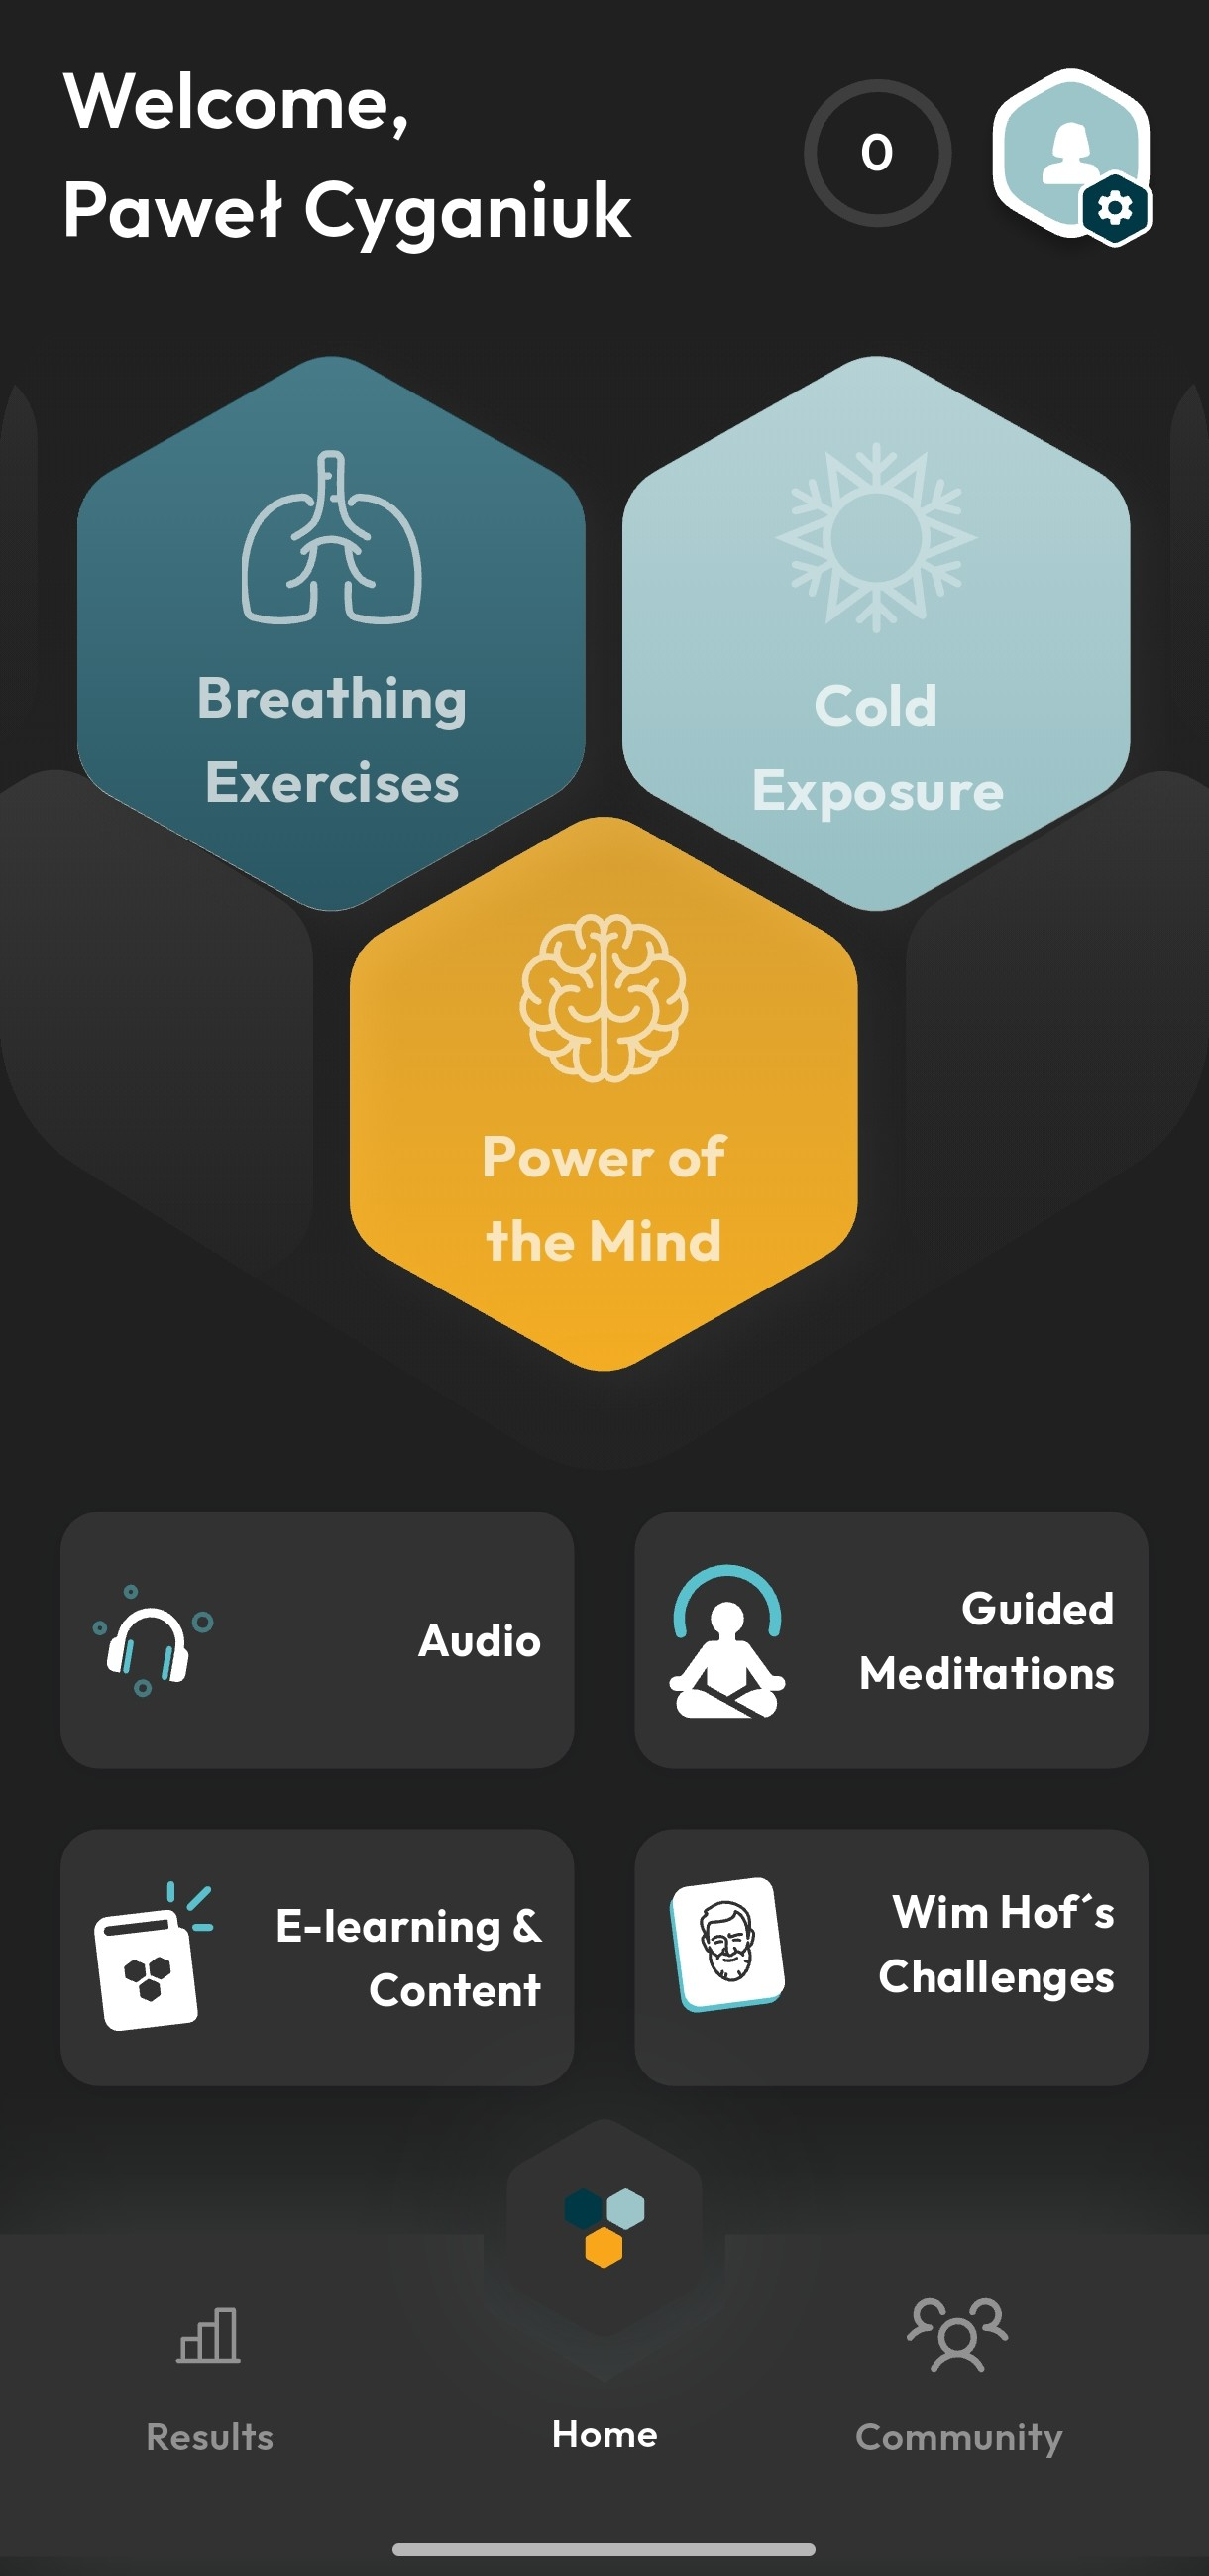
\includegraphics[width=0.27\textwidth,height=0.40\textheight,keepaspectratio]{obrazy/menu_wim.jpg}
    }
    \hfill
    \subfloat[Wizualizacja oddechu]{
        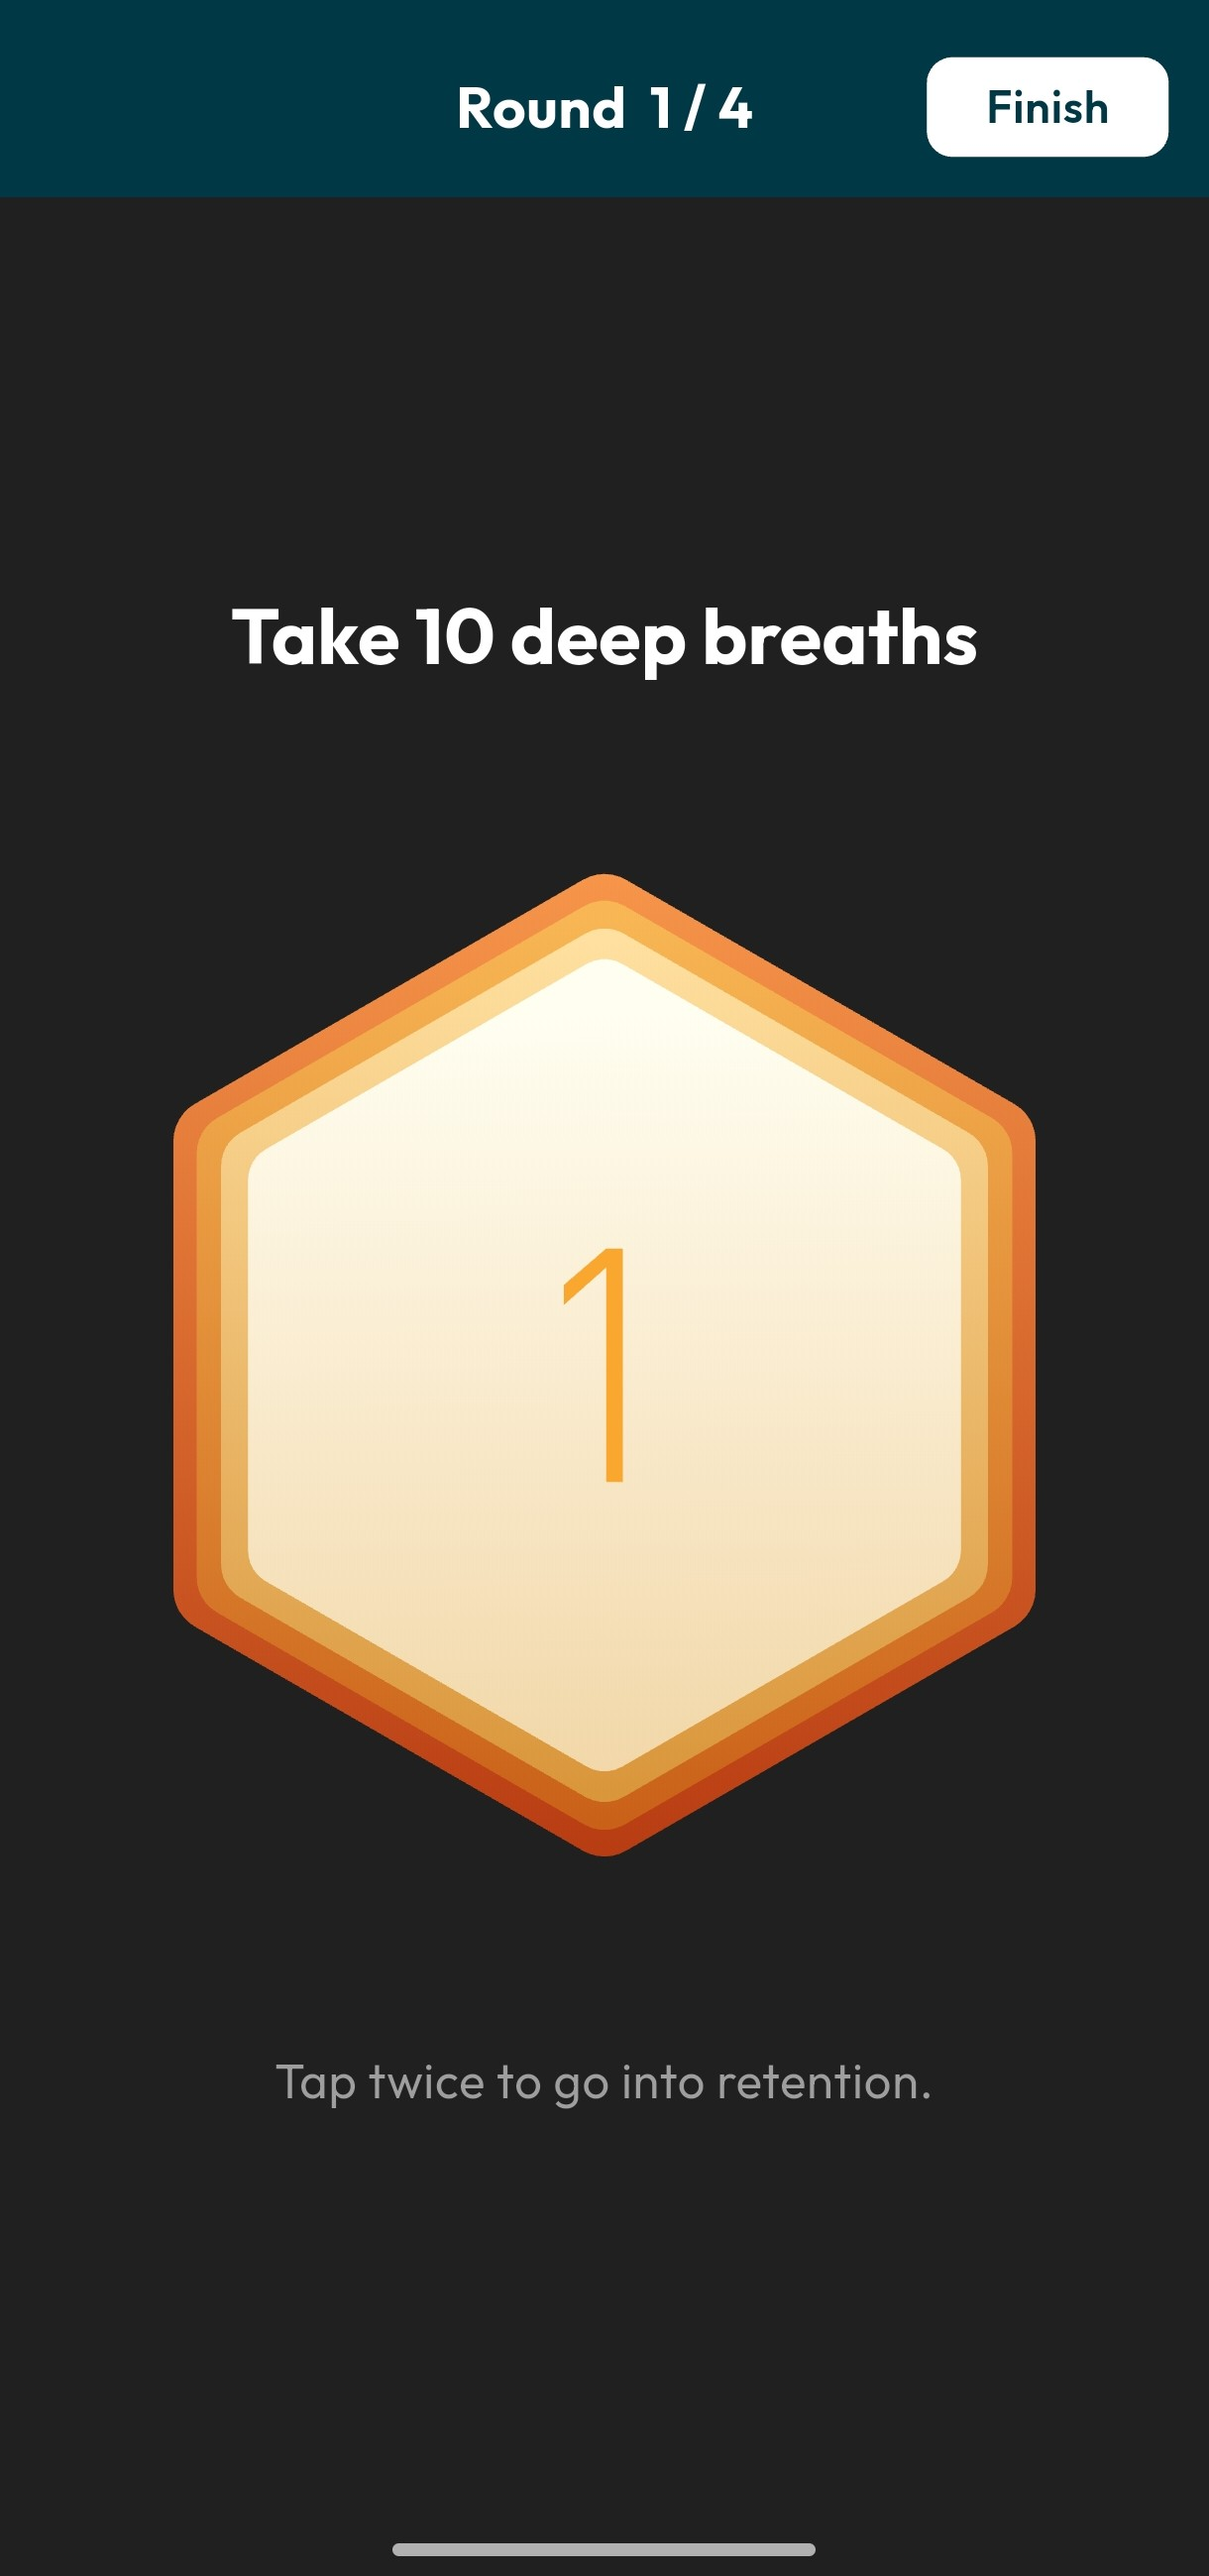
\includegraphics[width=0.27\textwidth,height=0.40\textheight,keepaspectratio]{obrazy/start_treningu_wim.jpg}
    }
    \hfill
    \subfloat[Wstrzymanie oddechu]{
        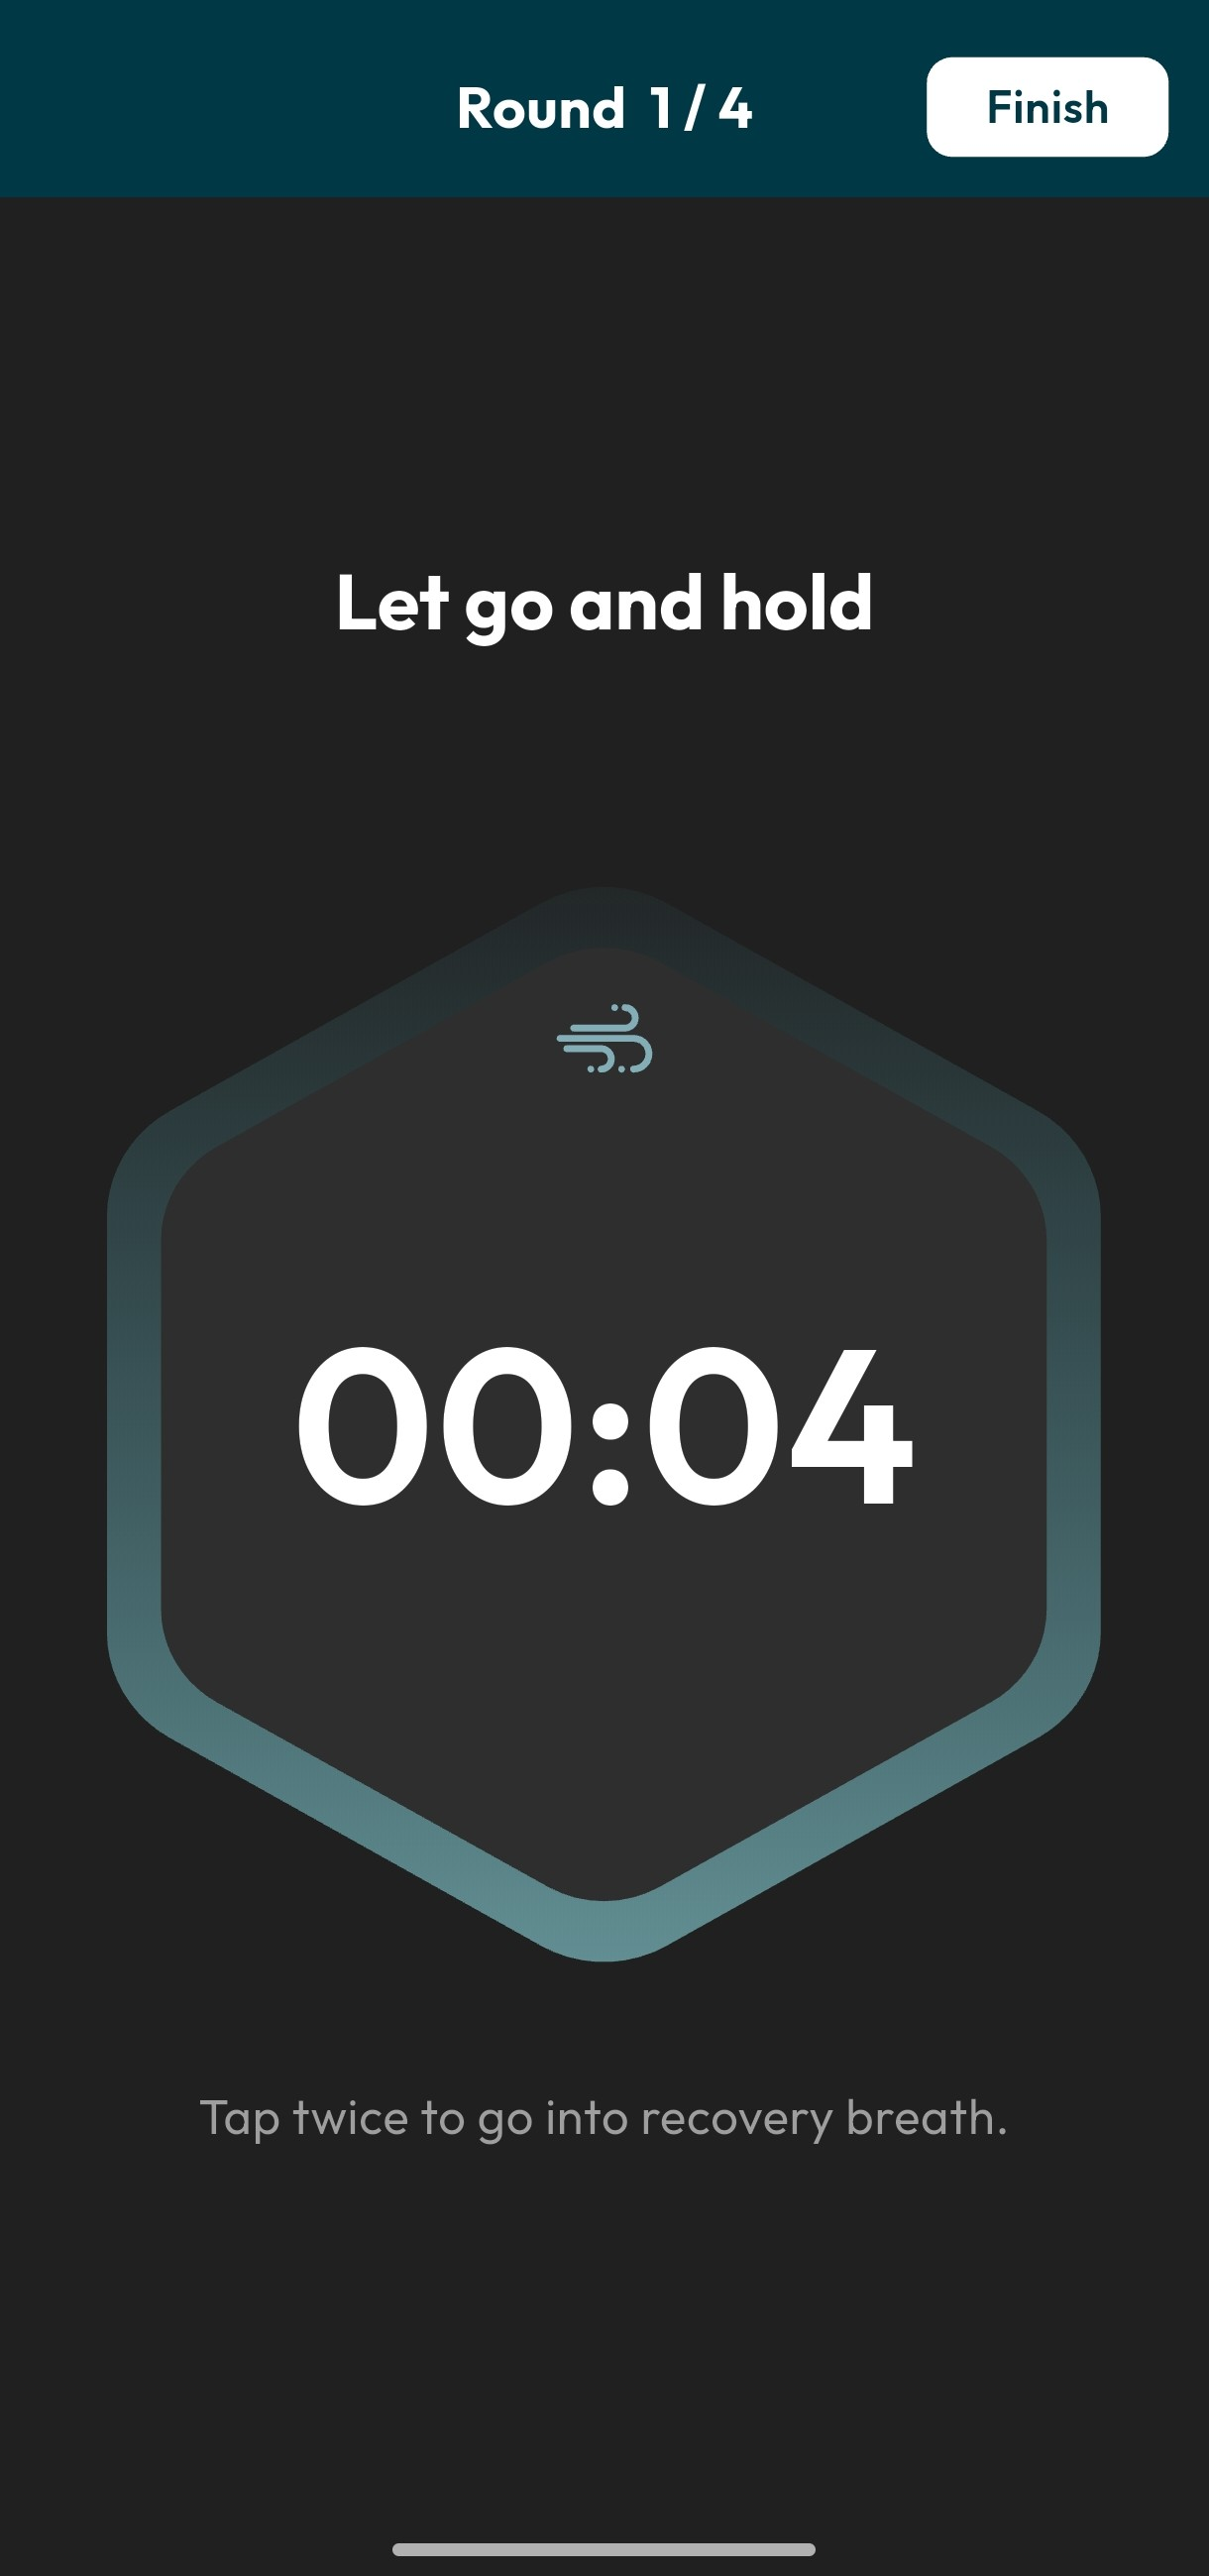
\includegraphics[width=0.27\textwidth,height=0.40\textheight,keepaspectratio]{obrazy/wstrzymanie_wim.jpg}
    }

    \caption{Zrzuty ekranu z aplikacji Wim Hof Method}
    \label{fig:wim_hof_method}
\end{figure}

Pomimo rozbudowanego systemu treningów aplikacja posiada istotne ograniczenia związane z personalizacją ćwiczeń. Użytkownik nie ma możliwości tworzenia w pełni własnych treningów ani swobodnego definiowania etapów sesji. Personalizacja ogranicza się jedynie do kilku podstawowych parametrów przygotowanych przez twórców aplikacji.
\subsubsection{Breathwrk}
Podobną aplikacją do wyżej wymienionej jest Breathwrk \cite{breathwrk2026}. W przeciwieństwie do Wim Hof Method, Breathwrk oferuje bardziej rozbudowaną bibliotekę treningów przeznaczonych do redukcji stresu, poprawy koncentracji, snu oraz zwiększania energii.

Istotnym elementem aplikacji są rozbudowane metody wizualizacji treningu. Podczas ćwiczeń użytkownik może korzystać z różnych animacji wyznaczających rytm oddechu, takich jak koło, linia czy animowane efekty immersyjne. Breathwrk kładzie większy nacisk na oprawę wizualną i dodatkowe bodźce, jak na przykład efekty świetlne, dźwięki tła czy wibracje telefonu synchronizowane z oddechem. Aplikacja umożliwia również korzystanie z instrukcji głosowych oraz ponowne uruchamianie treningu z wcześniej wybranymi ustawieniami.

Breathwrk oferuje także funkcje monitorowania aktywności użytkownika, takie jak statystyki treningów, poziomy rankingowe czy przypomnienia pomagające budować nawyk regularnych ćwiczeń. Podobnie jak w aplikacji Wim Hof Method, użytkownik może zapisywać ulubione treningi oraz śledzić swoje postępy.

\begin{figure}[h]
    \centering

    \subfloat[Menu aplikacji]{
        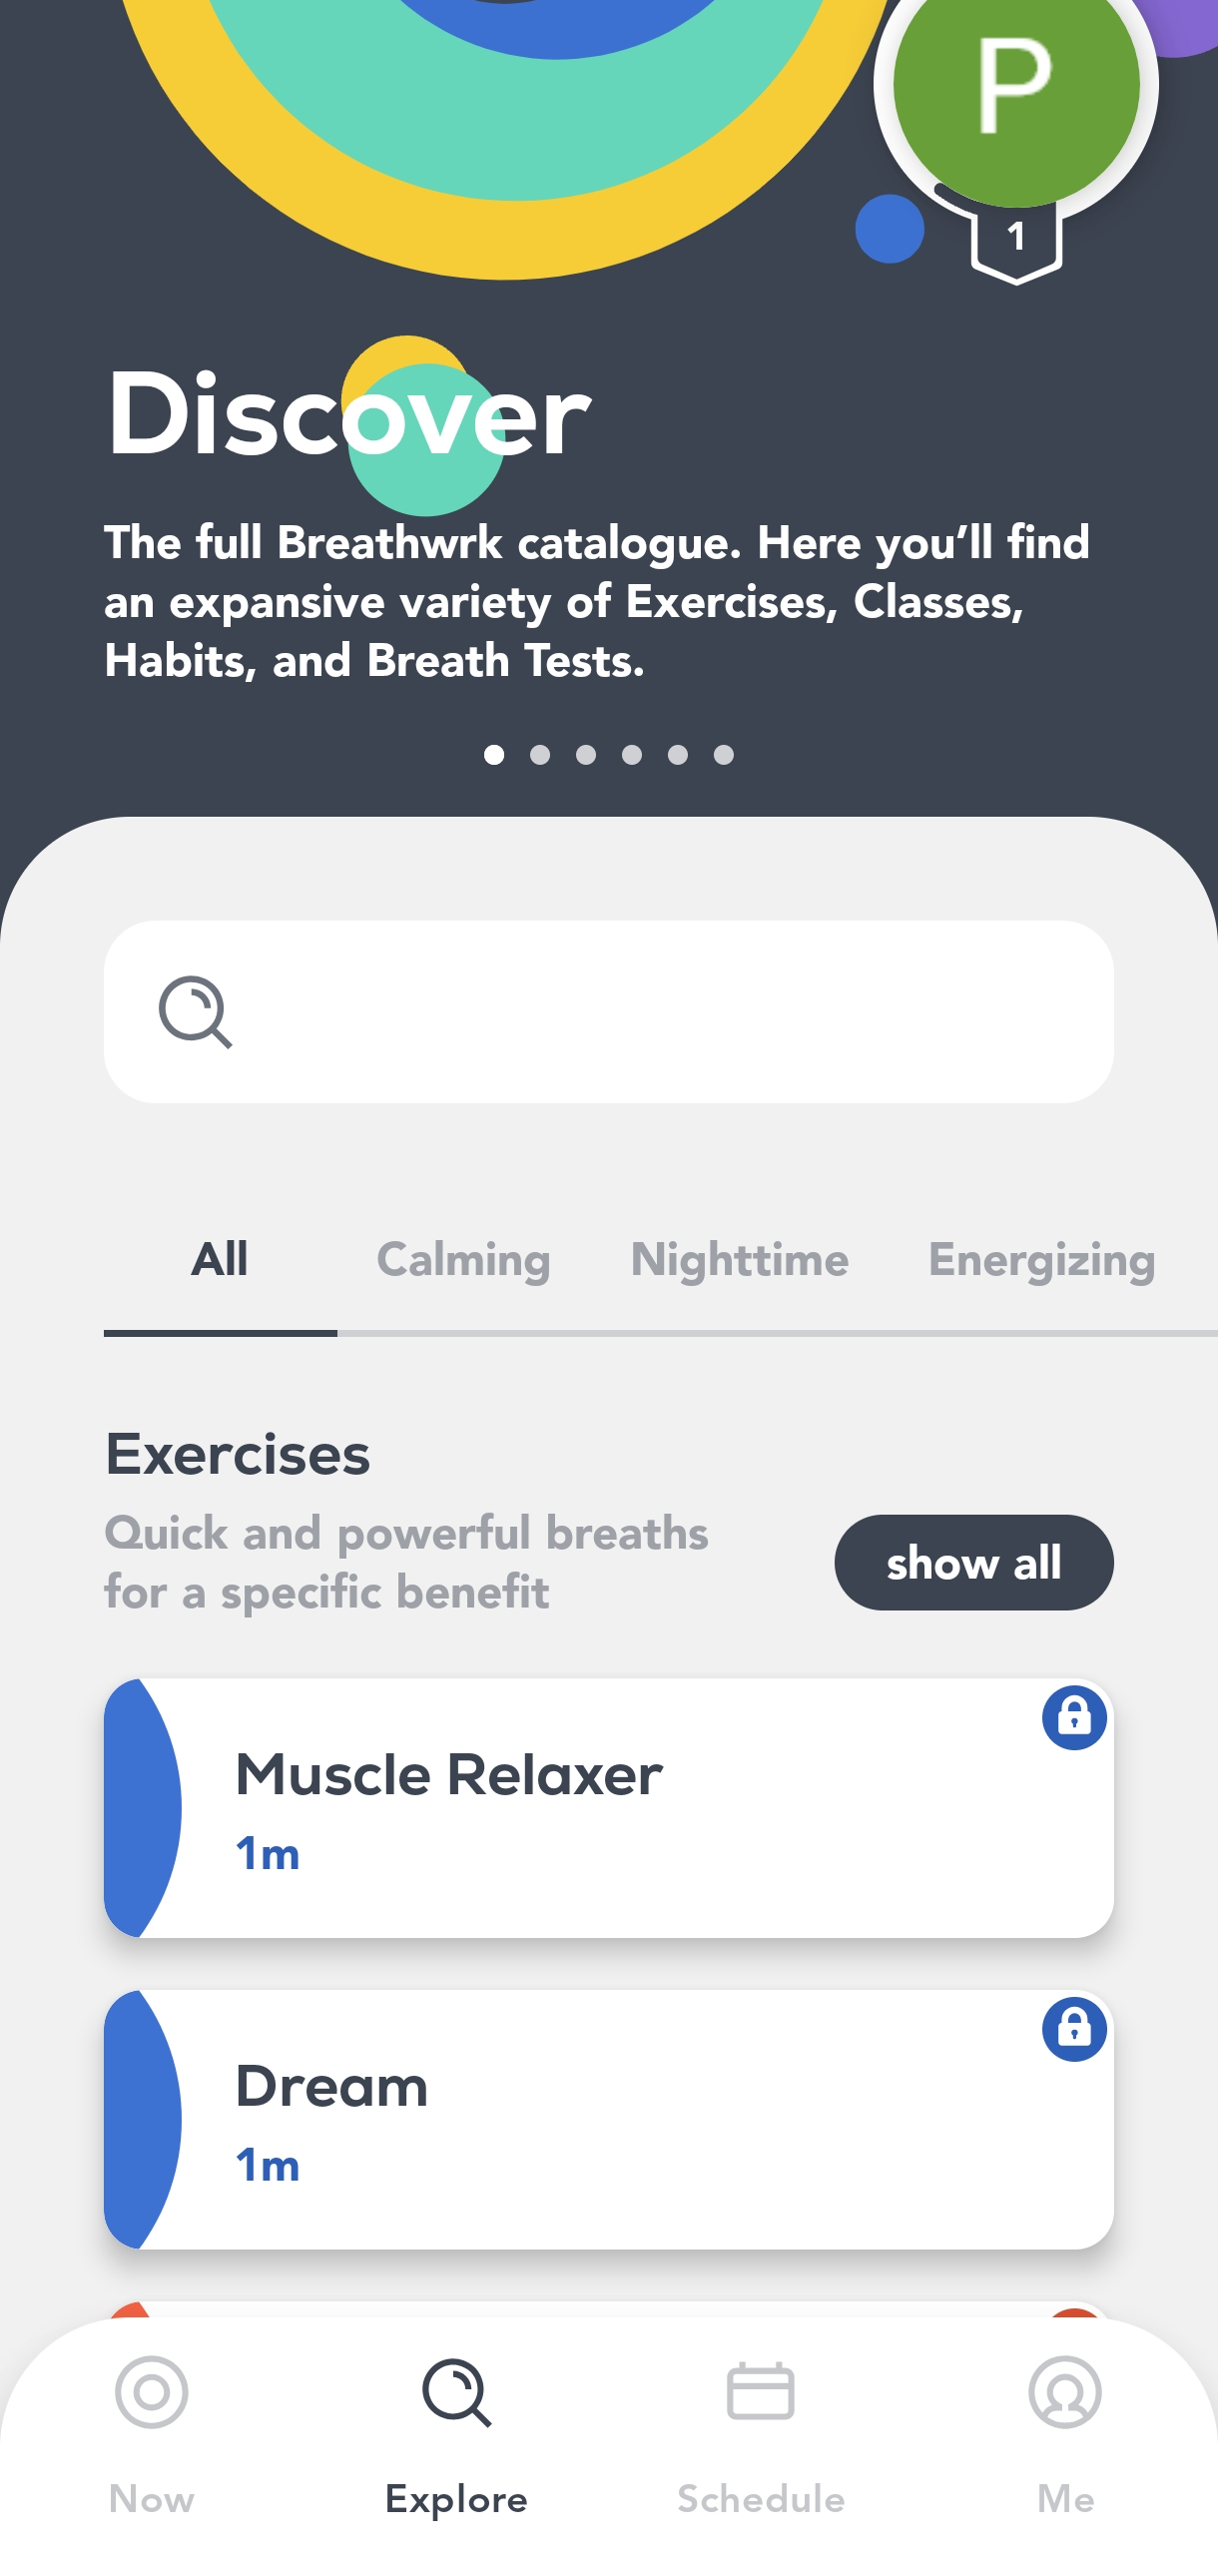
\includegraphics[width=0.27\textwidth,height=0.40\textheight,keepaspectratio]{obrazy/breathwrk_menu.jpg}
    }
    \hfill
    \subfloat[Standardowa wizualizacja oddechu]{
        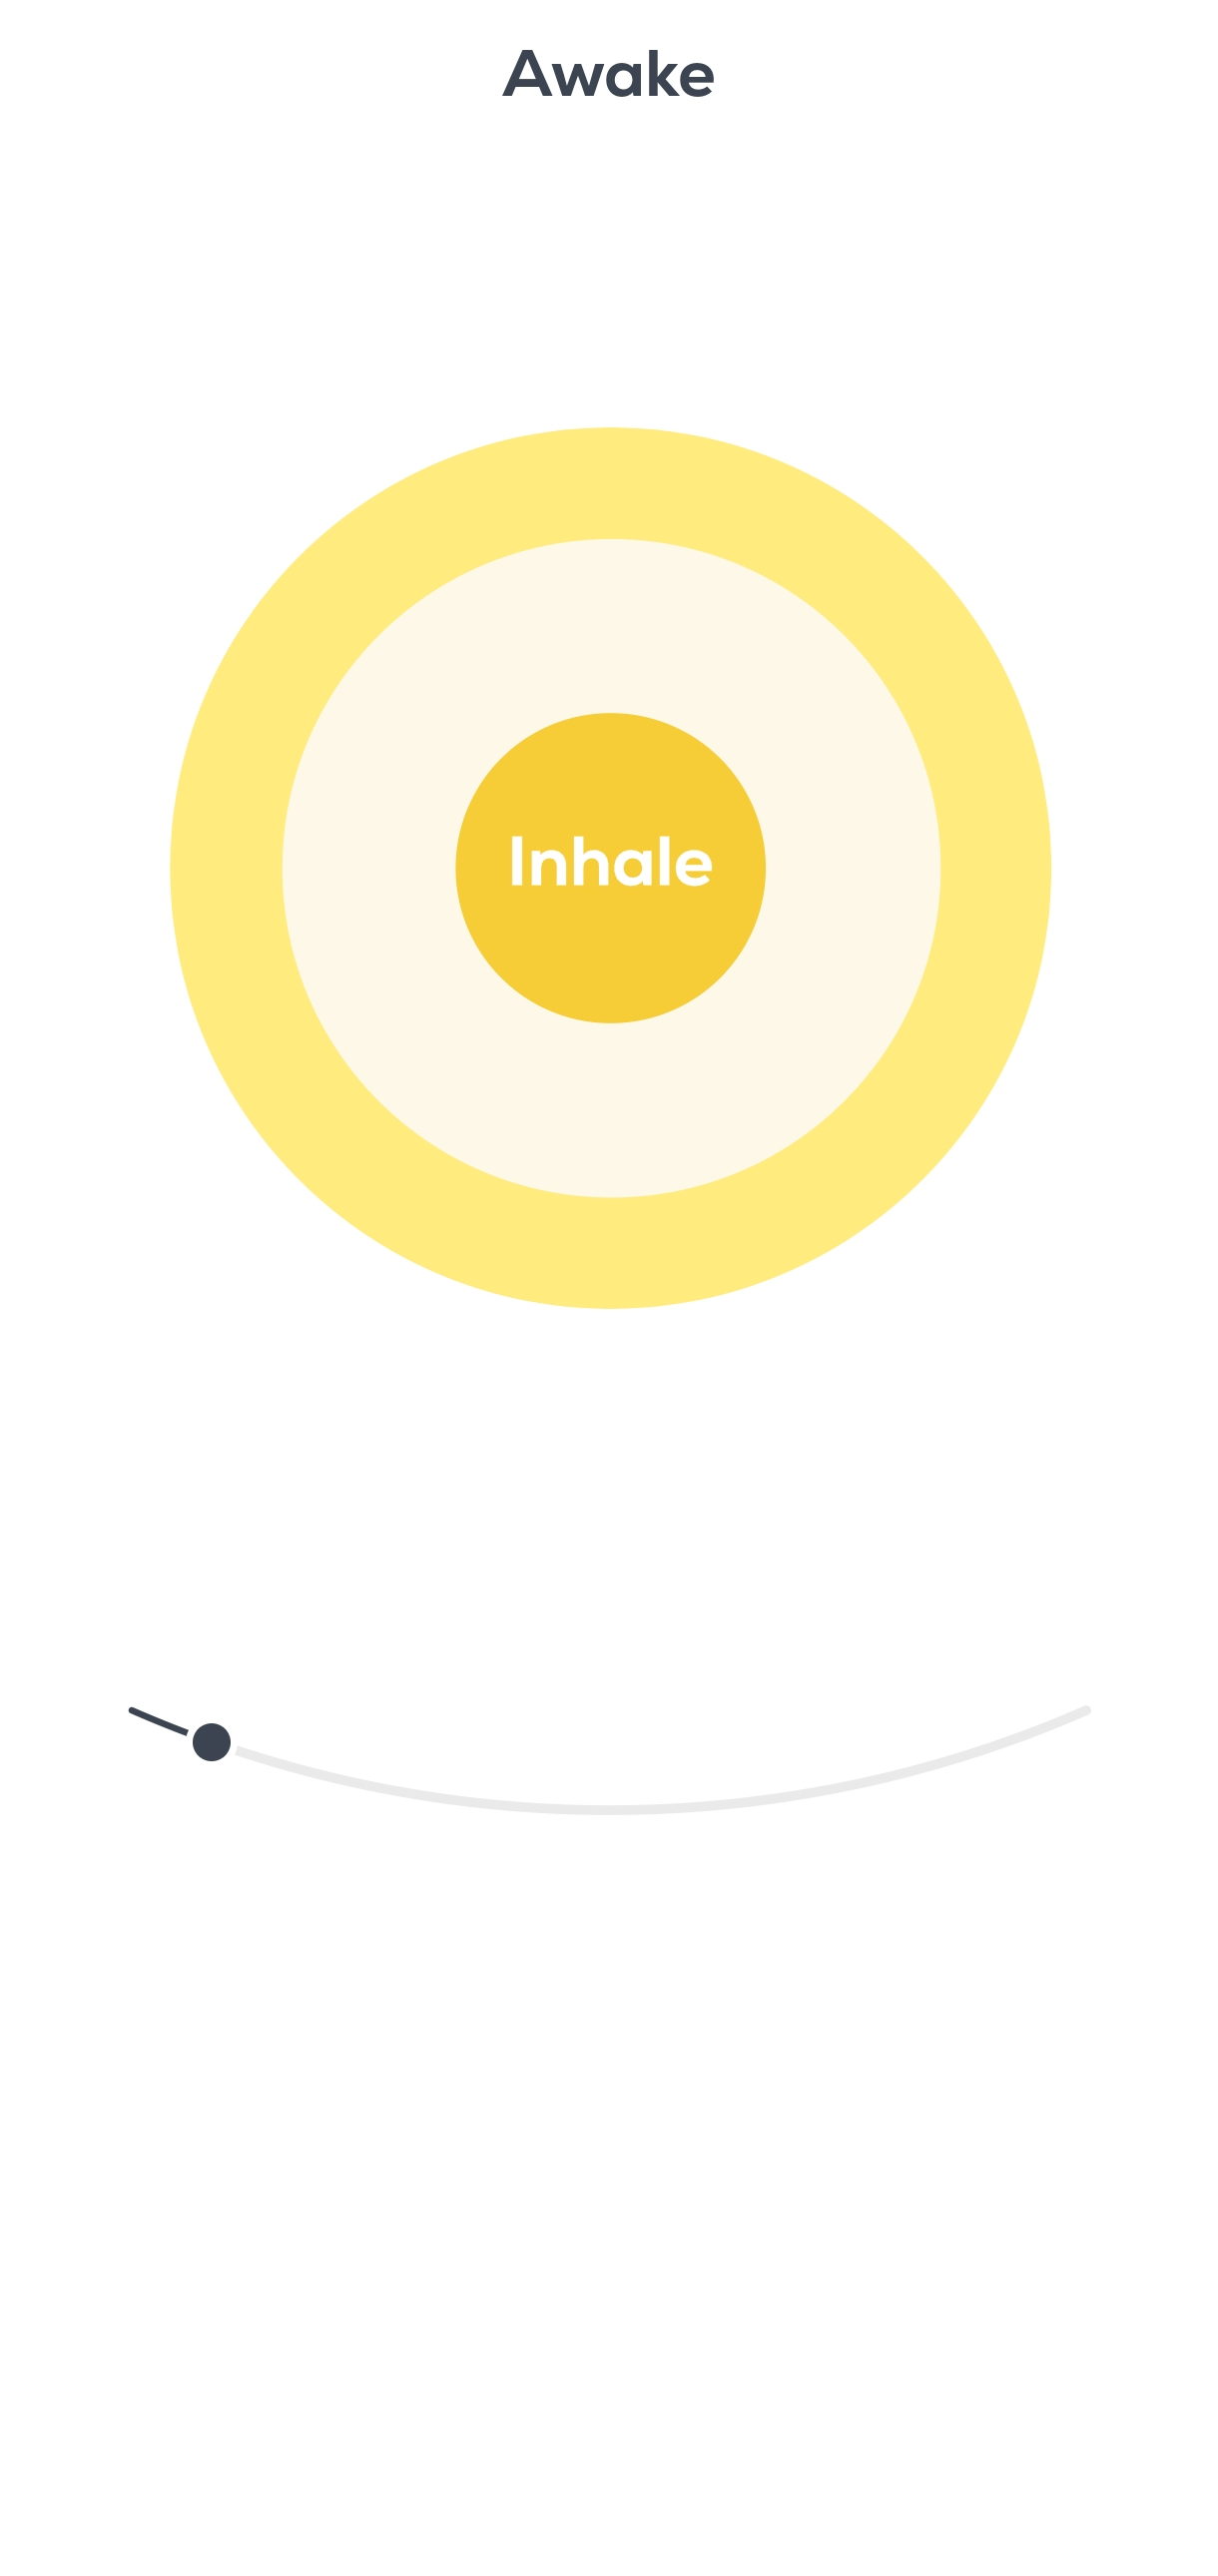
\includegraphics[width=0.27\textwidth,height=0.40\textheight,keepaspectratio]{obrazy/breathwrk_training_normal.jpg}
    }
    \hfill
    \subfloat[Immersywna wizualizacja oddechu]{
        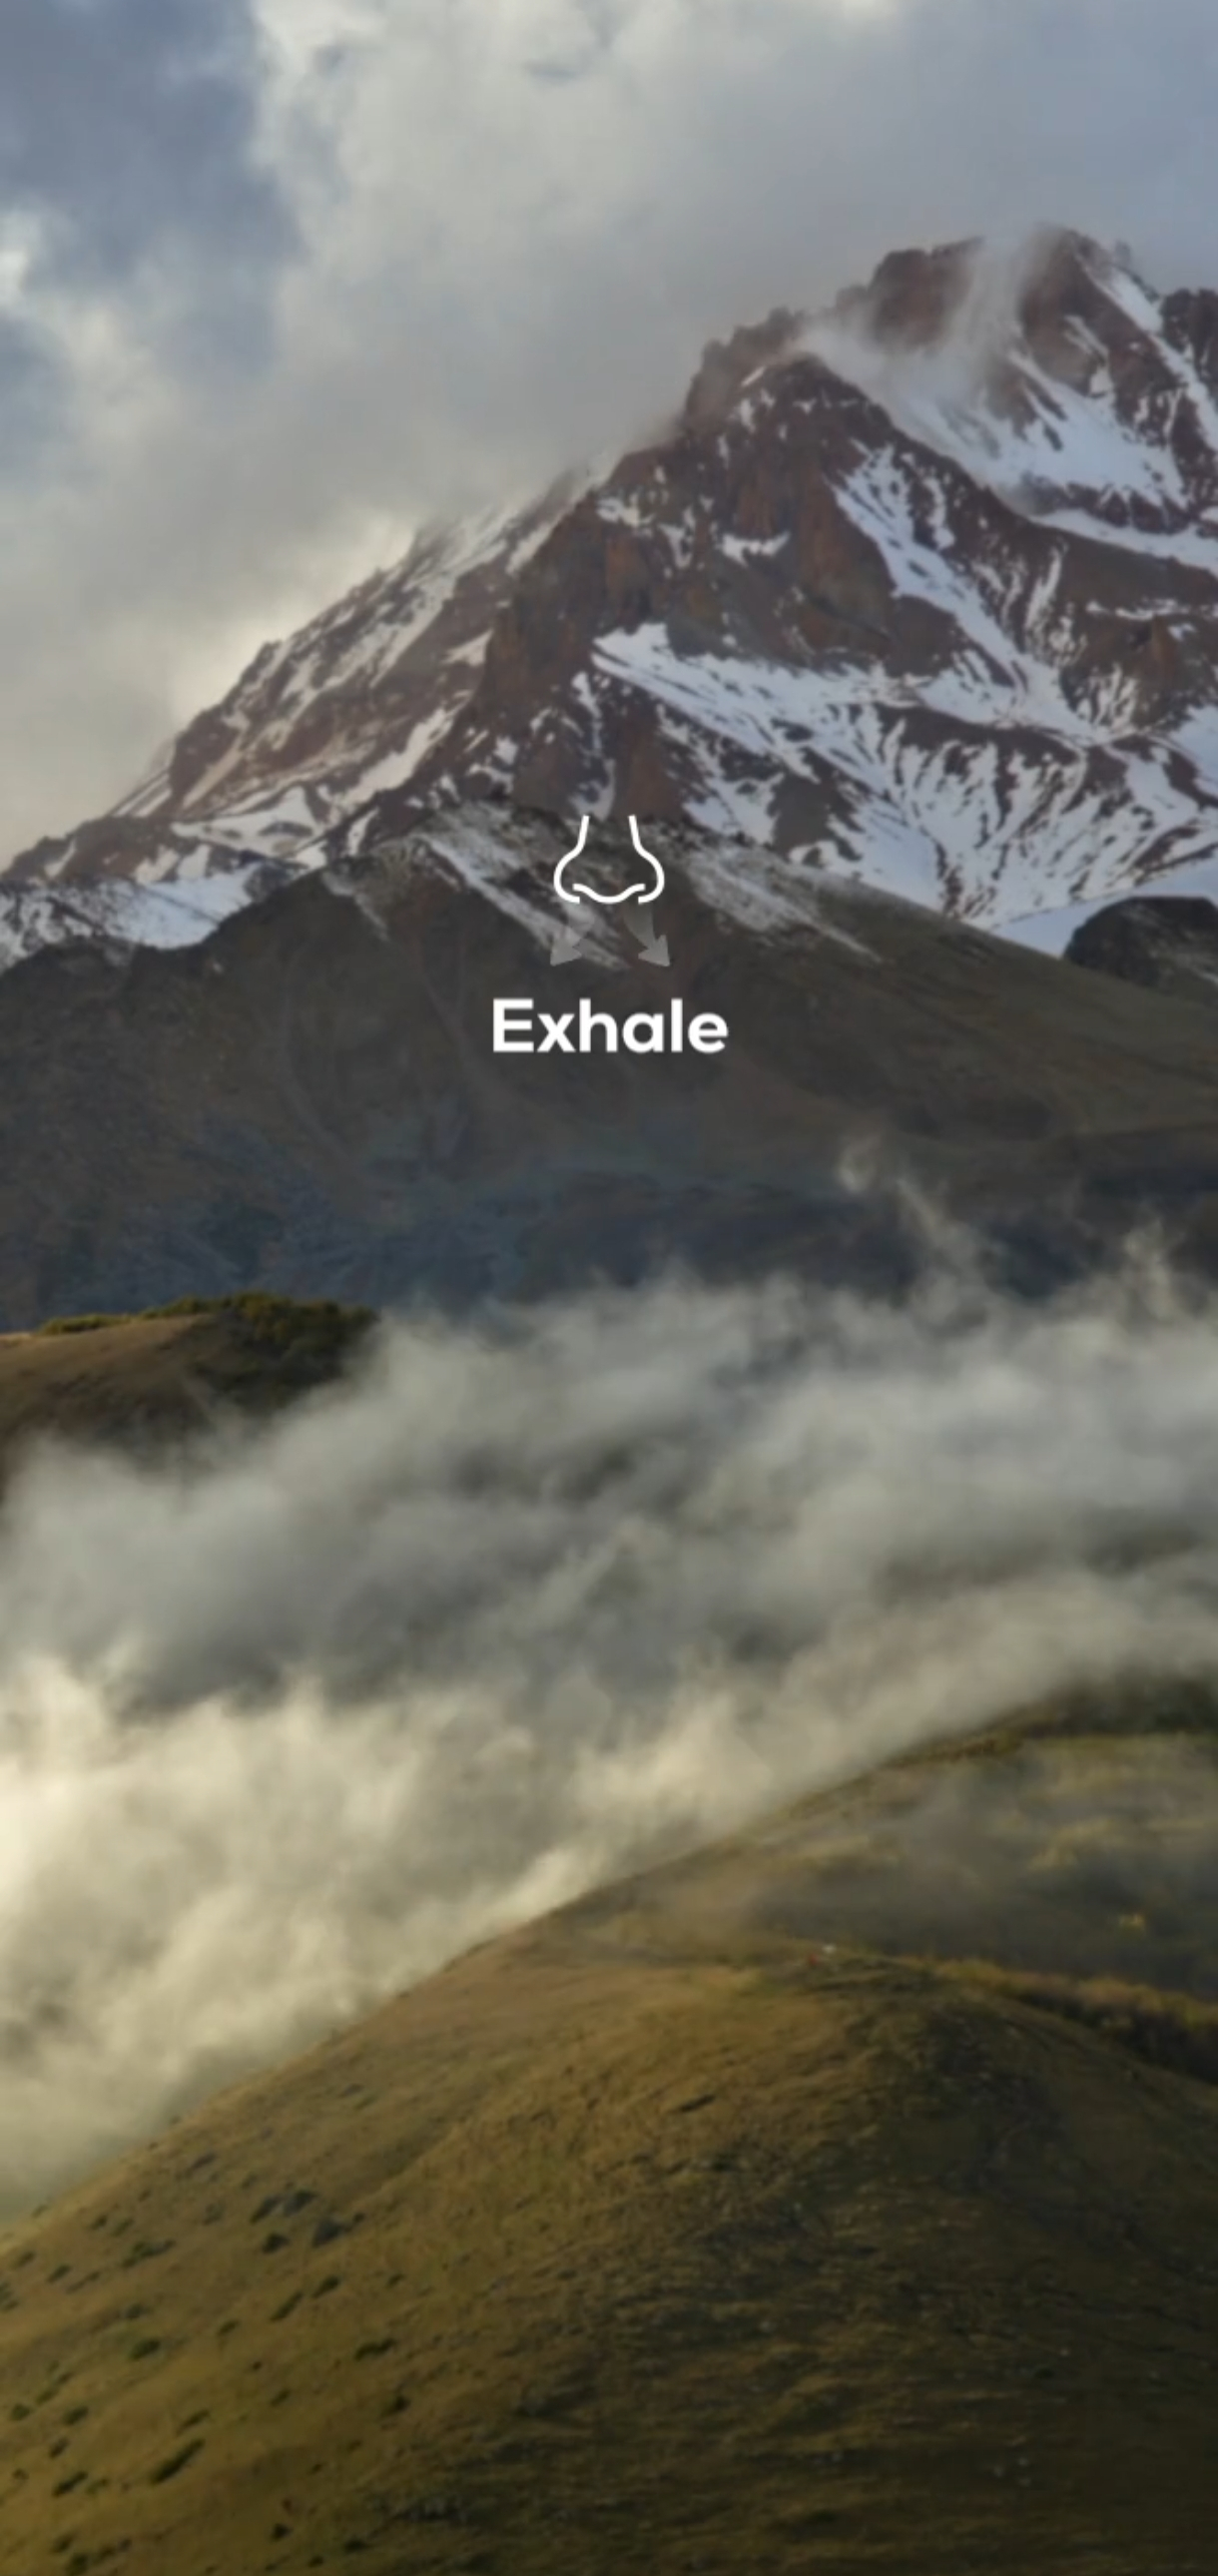
\includegraphics[width=0.27\textwidth,height=0.40\textheight,keepaspectratio]{obrazy/breathwrk_training_sky.jpg}
    }

    \caption{Zrzuty ekranu z aplikacji Breathwrk}
    \label{fig:breathwrk}
\end{figure}
Pomimo większego nacisku na warstwę wizualną i różnorodność gotowych treningów, aplikacja nadal posiada ograniczenia związane z personalizacją. Użytkownik nie może tworzyć własnych sesji oddechowych ani swobodnie definiować długości poszczególnych etapów ćwiczenia. Możliwa jest jedynie częściowa modyfikacja parametrów treningu, a część funkcji dostępna jest wyłącznie w wersji Premium.


\subsection{Aplikacje wspierające monitorowanie oddechu}
\subsubsection{Breeze}
Istotnym przełomem technologicznym w kontekście monitorowania oddechu jest rozwiązanie o nazwie Breeze \cite{10.1145/3369835}. Autorzy opracowali aplikację mobilną, która całkowicie eliminuje konieczność stosowania zewnętrznych urządzeń sensorycznych. Aplikacja wykorzystuje wyłącznie wbudowany w smartfon mikrofon do ciągłej detekcji faz oddechu użytkownika w czasie bliskim rzeczywistemu. Umożliwia ona realizację przetestowanego klinicznie wzorca oddechowego "4-2-4", składającego się z czterech sekund wdechu, dwóch sekund wydechu oraz czterech sekund pauzy, celując w indukcję oddechu z częstotliwością sześciu pełnych cykli na minutę. Aby zrealizować takie rozwiązanie w praktyce, konieczne było przezwyciężenie trudności związanych z niskim stosunkiem sygnału do szumu (SNR), zwłaszcza ze względu na niemal niesłyszalny dla mikrofonu dźwięk wdechu naturalnego.

Kluczowym elementem wkładu badawczego autorów pracy jest stworzenie bardzo dokładnego potoku przetwarzania sygnału akustycznego. Odebrany przez mikrofon dźwięk jest analizowany w jedno-sekundowych oknach. Na początku sygnał poddawany jest wstępnemu przetwarzaniu z użyciem filtrów pasmowo-przepustowych, a następnie, przy pomocy przesuwnych okien czasowych o długości 44 ms i nakładaniu 75\%, wyodrębniane są cechy częstotliwościowe, w tym charakterystyki w skali logMel oraz współczynniki melcepstralne (MFCC). Tak przygotowane dane wejściowe przekazywane są do dwuetapowego modelu rozpoznawania opartego o architekturę głębokich sieci neuronowych.  

\begin{figure}[h]
    \centering
    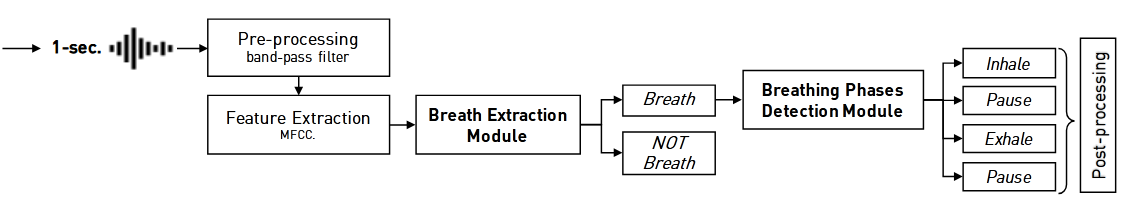
\includegraphics[width=1.0\linewidth]{obrazy/breeze_pipeline.png}
    \caption{Pipeline obróbki sygnału dźwiękowego aplikacji Breeze}
    \label{fig:breeze_pipeline}
\end{figure}

Proces przetwarzania sygnału dźwiękowego pozyskiwanego z mikrofonu urządzenia mobilnego został przedstawiony na Rysunku \ref{fig:breeze_pipeline}. Pierwszą warstwę detekcji stanowi Moduł Ekstrakcji Oddechu (BEM). Pełni on rolę zaawansowanej bramki kalibracyjnej, oddzielającej sygnał właściwy od dźwięków tła takich jak mowa, kaszel czy śmiech. Moduł BEM oparto o jednowarstwową splotową sieć neuronową (CNN) stosującą dziesięć filtrów, funkcję aktywacji ReLU oraz końcową klasyfikację klas za pomocą warstwy w pełni połączonej (FC) z funkcją softmax. Wyizolowane dzięki BEM ramki dźwiękowe zawierające poprawny sygnał oddechowy trafiają z kolei do Modułu Detekcji Faz (BPDM). Biorąc pod uwagę podobieństwo właściwości akustycznych wdechu i wydechu, autorzy odeszli od analizy niezależnych klatek dźwięku na rzecz analizy wzorców w czasie. Zastosowano tu dwukierunkową sieć z pamięcią długoterminową i krótko-terminową (BiLSTM), wzbogaconą o mechanizm uwagi. Mechanizm uwagi pozwala modelowi dynamicznie alokować "skupienie"~na tych fragmentach długiej sekwencji dźwiękowej, które niosą ze sobą największą wartość informacyjną w określeniu bieżącej fazy. Ostateczny wynik optymalizowany jest poprzez algorytm post-processingu w celu uniknięcia migotania fałszywych odczytów i zapewnienia płynnego interfejsu.  

Dla wytrenowania powyższych algorytmów konieczne było skompletowanie wysoce zróżnicowanego zbioru danych. Autorzy przeprowadzili sesję rejestracji danych z udziałem 43 uczestników, tworząc bazę ponad 2,76 miliona zdarzeń oddechowych. Aby system był uniwersalny i niezależny od specyfikacji sprzętowej konkretnego telefonu, próbki zbierano jednocześnie na czterech różnych urządzeniach mobilnych oraz dodatkowo na referencyjnym mikrofonie studyjnym. Dodatkowo użyty został bezprzewodowy pas mierzący ekspansję klatki piersiowej, pełniący funkcję fizjologicznego punktu odniesienia. Dane poddano półautomatycznemu etykietowaniu, gdzie oprócz informacji z sensora na ciele korzystano m.in. z filtru Savitzky'ego-Golay'a \cite{5888646} oraz algorytmu dekodowania Viterbiego do identyfikacji poszczególnych faz cyklu.  

% TU SKONCZYŁEM NA RAZIE

\begin{figure}[h]
    \centering
    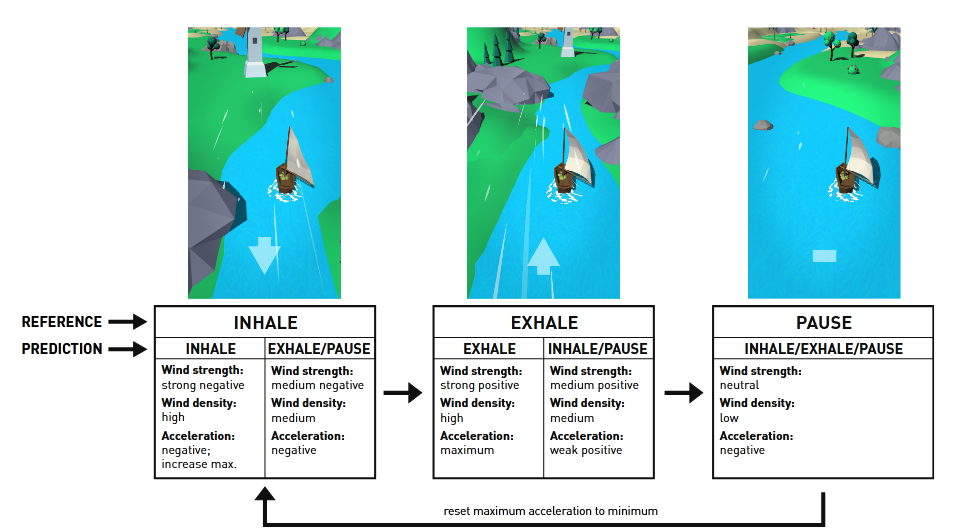
\includegraphics[width=0.80\linewidth]{obrazy/breeze_screen.png}
    \caption{Sposób działania aplikacji Breeze}
    \label{fig:breeze_workflow}
\end{figure}

Oprócz samego przetwarzania sygnałów, system Breeze kładzie również nacisk na element grywalizacji, który ma bezpośrednie przełożenie na monitorowanie treningu oraz satysfakcję i motywację końcowego użytkownika. Wygenerowane wyniki faz oddechu uruchamiają dynamiczny, wizualny moduł zbudowany w środowisku silnika Unity. Ćwiczenia przybierają formę sterowania żaglówką za pomocą wykrywania faz oddechu. Gdy system wykryje, że użytkownik poprawnie realizuje nałożony profil "4-2-4"~nagradza on gracza odpowiednim poruszeniem łódki i zachowaniem środowiska. Wdech napędza oraz generuje cząsteczki wiatru, podczas gdy wydech wydyma żagiel i gwarantuje płynne przyśpieszenie obiektu. Tego typu biofeedback w środowisku naturalnym stanowi ważną wartość empiryczną dla odbiorców, a także zwiększa ich zaangażowanie. Oprócz tego widać również, że sama kolorystyka aplikacji została dopasowana tak aby działała kojąco i~uspokajająco na użytkownika. 

Jeśli chodzi o wyniki samego modelu zaproponowanego przez autorów to ewaluacja wydajności technologicznej oraz testy kliniczne potwierdzają ogromny potencjał opisanego systemu. Moduł ekstrakcji (BEM) wytrenowany we wspartym głębokim uczeniem środowisku osiągnął precyzję AUC wynoszącą 0,92. Detektor poszczególnych faz oddechowych (BPDM) uzyskał wysoką w warunkach rzeczywistych skuteczność klasyfikacji na poziomie 75,5\%. Co więcej, złożony potok aplikacji wymaga zaledwie od 2,65 mln do ok. 10 mln operacji zmiennoprzecinkowych i w teście na telefonie z procesorem Snapdragon 845 wykazał opóźnienia detekcji na bardzo niskim poziomie 119 milisekund, umożliwiając płynne wyświetlanie animacji w 30 klatkach na sekundę przy jednoczesnej analizie dźwięku bez nadmiernego obciążania procesora.  

Dodatkowo, badanie pilotażowe na grupie 16 ochotników dowiodło mierzalnych, medycznych zalet działania omawianego rozwiązania. Korzystanie ze smartfona z aplikacją Breeze doprowadziło do znacznego obniżenia częstotliwości oddechów użytkowników (z poziomu ok. 12 oddechów spoczynkowo do pożądanych ok. 6 cykli na minutę). Rejestrowane równolegle wartości elektrokardiogramu (EKG) ujawniły statystycznie istotny i znaczny wzrost parametru wariancji tętna (HF-HRV) względem stanu bazowego. Były to wyniki wyższe, a także lepsze niż dla grupy kontrolnej, która podążała za prostą animacją na ekranie niezawierającą aktywnego biofeedbacku. Z~perspektywy ewaluacji UX, interaktywna koncepcja przewyższyła standardowe metody niemal we wszystkich wymiarach, takich jak:
\begin{itemize}
    \item podwyższone uczucie immersji,
    \item dobrze odczuwalna responsywność aplikacji,
    \item pozytywne doświadczenie z używania aplikacji.
\end{itemize} 

Podsumowując, choć system Breeze stanowi interesujący przykład wykorzystania uczenia maszynowego w monitorowaniu parametrów życiowych, jego praktyczna użyteczność w warunkach rzeczywistych budzi pewne zastrzeżenia. Zaproponowana architektura oparta na sieciach splotowych i rekurencyjnych oraz pozyskiwaniu sygnału z mikrofonu samego urządzenia wykazuje zadowalającą skuteczność przede wszystkim w kontrolowanym środowisku, co może znacząco ograniczać jej niezawodność w obecności dynamicznego szumu otoczenia czy różnych specyfikacji mikrofonów w tańszych urządzeniach mobilnych.

Kluczowym problemem z perspektywy dalszego rozwoju tej technologii oraz transparentności badań naukowych jest fakt, że autorzy nie udostępnili ani wykorzystanego zbioru danych, ani kodu źródłowego algorytmów. Brak dostępu do tych zasobów uniemożliwia niezależną weryfikację przedstawionych wyników oraz utrudnia replikację badań w innych ośrodkach naukowych.
\subsubsection{BreathTrack}
Głównym problemem większości współczesnych systemów akustycznego monitorowania oddechu często jest bariera związana z trudnością w pozyskiwaniu wysokiej jakości etykietowanych danych treningowych. O ile faza wydechu jest zazwyczaj wyraźnie słyszalna dla mikrofonów wbudowanych w smartfony, o tyle faza wdechu podczas swobodnego, regularnego oddychania jest często niemal niesłyszalna, co uniemożliwia precyzyjne ręczne adnotowanie nagrań. Jednym z istniejących rozwiązań jest system BreathTrack \cite{10.1145/3478123}, zaproponowany przez zespół badawczy pod kierownictwem B. Islam, który jako pierwszy wprowadza paradygmat uczenia opartego na nieoznaczonych danych akustycznych dla oddechu spoczynkowego.

Kluczowym wkładem autorów jest opracowanie architektury wykorzystującej między modalnościowy transfer wiedzy, opartej na metodologii szkolenia Nauczyciel-Uczeń. Pozwala ona na ustalenie kluczowych wzorców oddechowych, takich jak frakcyjny czas wdechu czy stosunek wdechu do wydechu, bez konieczności ręcznego etykietowania sygnału audio. Główna innowacja BreathTrack polega na założeniu, że rzetelną wiedzę o fazach oddechu można pozyskać z innej domeny sensorycznej smartfona takiej jak czujniki inercyjne. W taki sposób pozyskany sygnał użyty został do automatycznego nadzorowania procesu uczenia modelu akustycznego.

W warstwie przetwarzania wstępnego i pozyskiwania etykiet, BreathTrack implementuje model Nauczyciela, który nie jest siecią uczenia głębokiego, lecz zaawansowanym algorytmem przetwarzania sygnału. Kiedy urządzenie znajduje się na klatce piersiowej użytkownika, system analizuje dane z akcelerometru i żyroskopu, wybierając oś o największej okresowości za pomocą transformaty Fouriera. Następnie wykorzystując filtr Savitzky'ego-Golay'a \cite{5888646} oraz post-processing oparty na filtrze Kalmana, system precyzyjnie identyfikuje fizyczne rozszerzanie i~kurczenie się klatki piersiowej. W ten sposób generowane są idealne etykiety czasowe dla faz wdechu i wydechu, które posłużą do oceny równolegle nagrywanego sygnału z mikrofonu.

\begin{figure}[h]
\centering
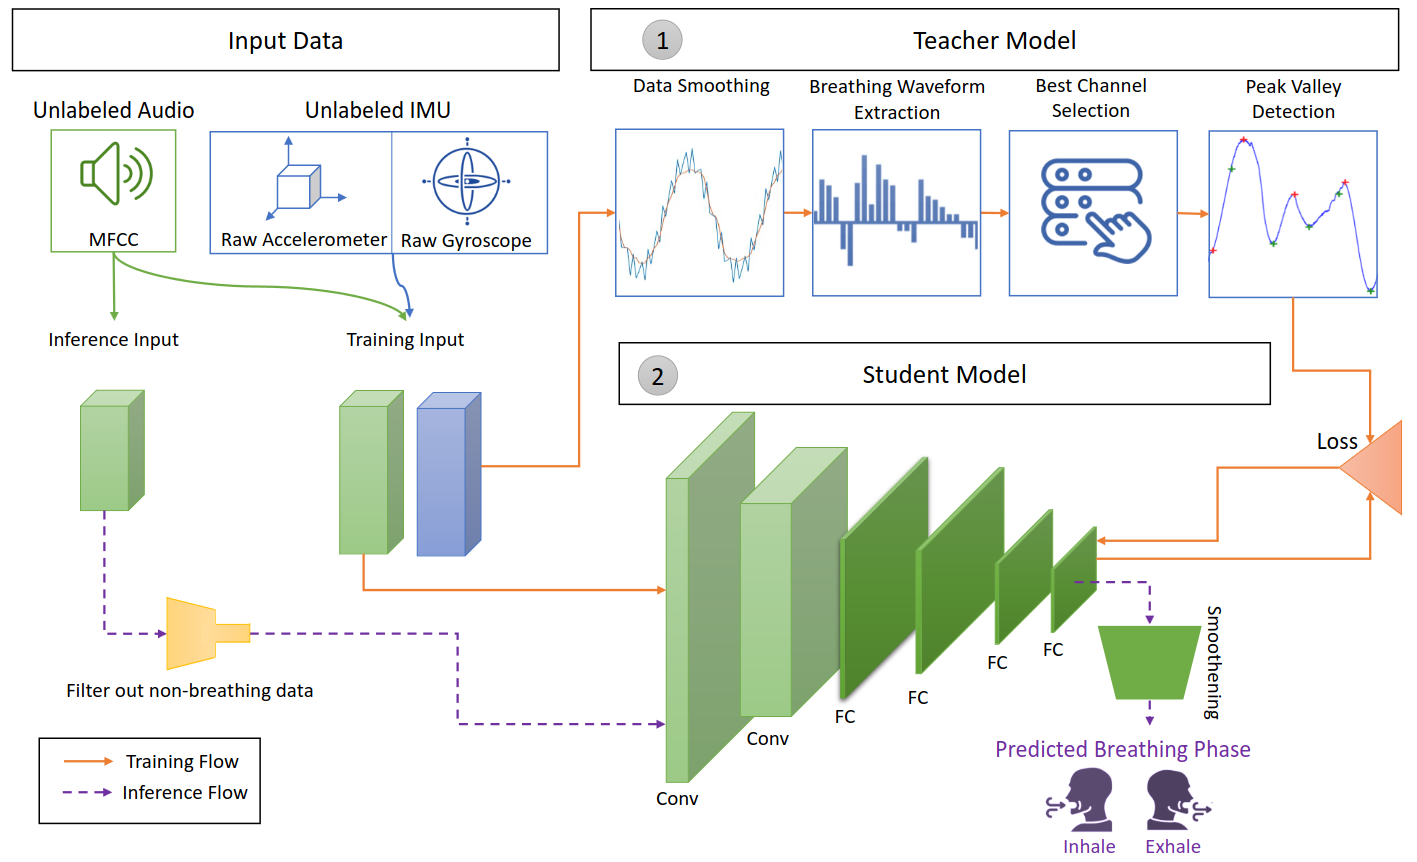
\includegraphics[width=0.90\linewidth]{obrazy/breathtrack_training_pipeline.png}
\caption{Potok treningu modelu BreathTrack, wykorzystujący architekturę Nauczyciel-Uczeń}
\label{fig:breathtrack_training_pipeline}
\end{figure}

Z kolei model predykcyjny dedykowany do docelowego działania opiera się wyłącznie na lekkiej, jednowymiarowej strukturze splotowej. Na wejście sieci trafiają 500 ms ramki dźwięku przetworzone do postaci współczynników melcepstralnych (MFCC). Architektura sieci składa się z dwóch warstw splotowych z normalizacją wsadową i 40-procentowym mechanizmem dropout. Następnie sygnał trafia do trzech warstw w pełni połączonych (FC) zakończonych funkcją aktywacji Sigmoid do klasyfikacji binarnej. Przez to że zrezygnowano tu ze struktur rekurencyjnych, w celu zachowania długofalowej spójności fizjologicznej autorzy zastosowali zewnętrzny algorytm wygładzania w fazie post-processingu. Analizuje on sąsiadujące segmenty czasowe i koryguje anomalie takie jak pojedynczy wdech wykryty w środku długiego wydechu znacząco poprawiając stabilność predykcji.

Ewaluacja systemu została przeprowadzona na zróżnicowanym zbiorze danych, obejmującym sesje nagraniowe w różnych pozycjach ciała i przy zmiennym natężeniu hałasu tła. Wyniki eksperymentalne wskazują, że BreathTrack osiąga dokładność w estymacji częstotliwości oddechu oraz granic faz oddechowych na poziomie porównywalnym z systemami w pełni nadzorowanymi, mimo braku dostępu do manualnych etykiet audio podczas treningu. Autorzy wykazali, iż błąd bezwzględny (MAE) w wyznaczaniu biomarkerów jest minimalny, co pozwala na wykorzystanie aplikacji do długofalowego monitorowania zdrowia, np. w wykrywaniu bezdechu sennego czy monitorowaniu stanów lękowych.

Z perspektywy projektowania systemów monitorujących oddech, BreathTrack rozwiązuje problem skalowalności. Po wytrenowaniu, model Ucznia jest w stanie analizować unikalną sygnaturę dźwiękową oddechu wyłącznie z mikrofonu, bez konieczności zakładania dodatkowych sensorów.

Należy jednak zauważyć pewne ograniczenia metodologiczne, które, podobnie jak w przypadku innych rozwiązań z tego segmentu, mogą wpływać na końcową ocenę pracy. Mianowicie autorzy nie zdecydowali się na upublicznienie kodu źródłowego ani zbioru danych, na którym przeprowadzano badania. Ogranicza to możliwość przeprowadzenia niezależnych testów porównawczych i utrudnia weryfikację odporności modelu na specyficzne, rzadkie artefakty akustyczne. Podsumowując, choć model jest w stanie wykryć nawet cichy oddech, jego wydajność w skrajnie głośnych środowiskach miejskich wciąż pozostaje obszarem wymagającym dalszego dostosowania.
\begin{comment}
Współczesne systemy mHealth kładą nacisk na interaktywność. Badania nad aplikacjami takimi jak te opisane w \textit{JMIR mHealth uHealth (doi:10.2196/63512)} oraz systemy typu \textbf{Breeze} (ACM, 10.1145/3369835), pokazują, że biofeedback oddechowy znacząco redukuje stres i poprawia uważność. Różnica między tymi rozwiązaniami a projektem dyplomowym polega na stopniu automatyzacji wykrywania faz – wiele rozwiązań komercyjnych wymaga ręcznego synchronizowania oddechu z animacją, podczas gdy niniejsza praca stawia na automatyczną detekcję.
\end{comment}
\subsection{Efektywne metody wizualizacji przebiegu treningu}
Kolejnym zagadnieniem w projektowaniu aplikacji wspierających treningi oddechowe jest sposób przekazywania użytkownikowi instrukcji dotyczących tempa i fazy oddechu. Tradycyjne metody wywodzące się z nagrań audio, opierają się wyłącznie na komendach głosowych. Obecnie popularniejszym podejściem są jednak metody wizualizujące oddech oraz przebieg treningu. Takie podejście zostało przebadane w artykule \textit{Evaluating mobile apps for breathing training: The effectiveness of visualization} \cite{chittaro2014evaluating}.

W ramach przeprowadzonych badań porównano trzy paradygmaty interfejsów aplikacji do treningu oddechowego. Każdy wariant został przetestowany dla treningu o docelowej częstotliwości sześciu cykli na minutę. Pierwszy z nich, wykorzystywał wyłącznie instrukcje głosowe z odliczaniem czasu trwania faz wdechu i wydechu. Następnie przebadano wariant widoczny na rysunku \ref{fig:sphere}, który integrował komunikaty audio z~pulsującą sferą, która rosła z wdechem, a także malała z wydechem, zmieniając przy tym kolor odpowiednio na zielony i czerwony. Trzeci wariant reprezentował podejście oparte na fali, w którym proces oddechu był wizualizowany jako przesuwająca się po ekranie fala trójkątna, z wyraźnie zaznaczonym bieżącym punktem cyklu, który widoczny jest na rysunku \ref{fig:wave}.

\begin{figure}[h]
    \centering
    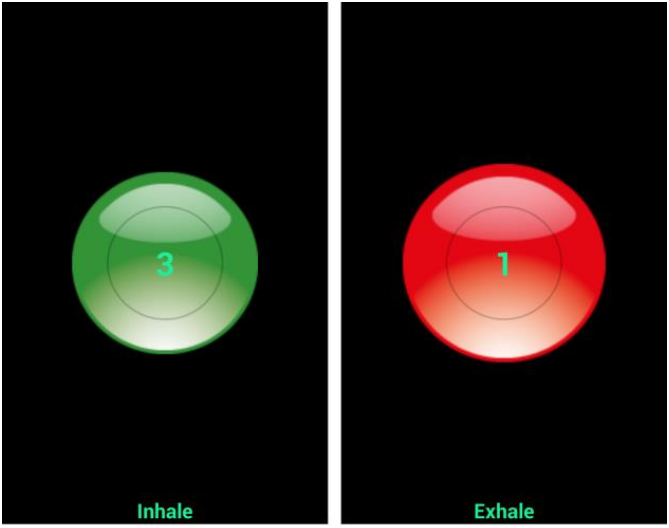
\includegraphics[width=0.80\linewidth]{obrazy/bubble.png}
    \caption{Wizualizacja treningu za pomocą sfery}
    \label{fig:sphere}
\end{figure}

\newpage

\begin{figure}[h]
    \centering
    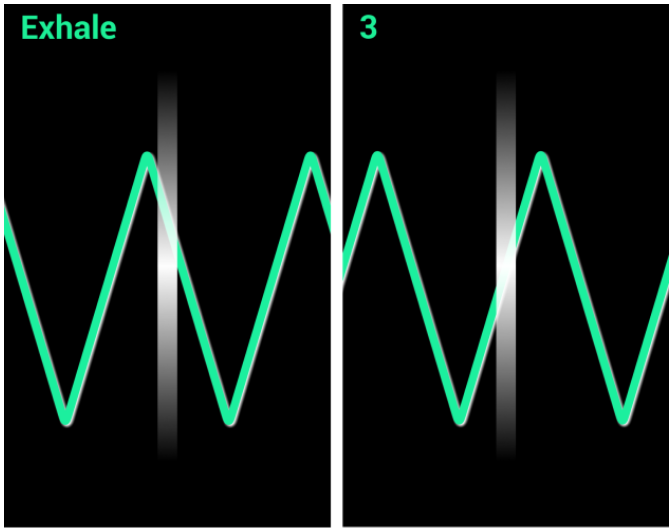
\includegraphics[width=0.80\linewidth]{obrazy/wave.png}
    \caption{Wizualizacja treningu za pomocą fali}
    \label{fig:wave}
\end{figure}

Ewaluacja przeprowadzona na grupie 68 uczestników przy użyciu klinicznej aparatury pomiarowej (m.in. sensorów objętości klatki piersiowej, czujników tętna oraz aktywności elektrodermalnej) jednoznacznie wykazała przewagę interfejsów wykorzystujących zaawansowaną wizualizację graficzną. Aplikacja wykorzystująca wizualizację fali pozwoliła użytkownikom na osiągnięcie statystycznie istotnie głębszego oddechu w docelowym paśmie częstotliwości w porównaniu do aplikacji bazującej wyłącznie na dźwięku.  

\begin{figure}[h]
    \centering
    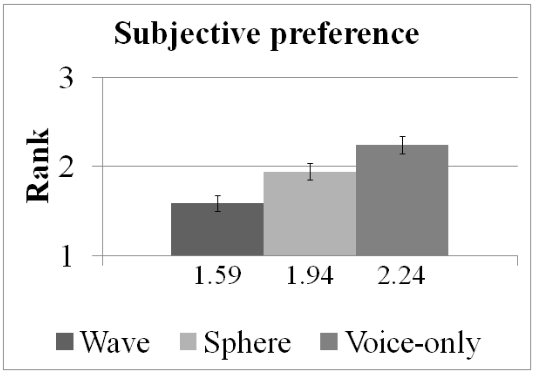
\includegraphics[width=0.5\linewidth]{obrazy/sub-pref.png}
    \caption{Porównanie wyników preferencji użytkowników w stosunku do sposoby wizualizacji treningu}
    \label{fig:sub-pref}
\end{figure}

Zaletą wizualizacji opartych na fali jest dostarczanie szerszego kontekstu czasowego ćwiczenia. W przeciwieństwie do pulsujących sfer lub komend głosowych, które informują jedynie o bieżącym stanie, fala na ekranie pozwala użytkownikowi obserwować zarówno aktualną, jak i~nadchodzącą fazę oddechu. Pozwala to na lepsze zaplanowanie objętości wdychanego powietrza i płynniejsze przejścia między fazami eliminując problem nagłego zatrzymywania oddechu przed końcem danej fazy z powodu braku pojemności płuc. Ponadto, jak wynika z rysunku \ref{fig:sub-pref} z~perspektywy subiektywnej oceny, użytkownicy ocenili wariant z falą jako najbardziej efektywny zarówno w kontekście nauki oddychania czy osiągania stanu relaksacji, wskazując go jako interfejs najbardziej preferowany.  

Wyniki te mają fundamentalne znaczenie dla projektowania systemów wspomagania treningów oddechu. Dowodzą one, że prawidłowo zaprojektowany wizualny biofeedback nie rozprasza użytkownika, lecz znacząco podnosi fizjologiczną skuteczność terapii. Wskazują również optymalny kierunek rozwoju interfejsów użytkownika, sugerując implementację grafów prezentujących ciągłość i historię cyklu oddechowego zamiast prostych animacji geometrycznych.
\begin{comment}
Wybór metody wizualizacji ma kluczowy wpływ na skuteczność treningu. Zgodnie z badaniami opublikowanymi w \textit{Computers in Human Behavior} (https://doi.org/10.1016/j.chb.2014.07.049):
\begin{itemize}
    \item \textbf{Wizualizacje abstrakcyjne (np. rozszerzające się koło):} Są najbardziej intuicyjne i najmniej obciążające poznawczo.
    \item \textbf{Wizualizacje oparte na naturze:} Zwiększają zaangażowanie i poczucie relaksacji (np. falowanie wody).
    \item \textbf{Wykresy w czasie rzeczywistym:} Najlepsze dla zaawansowanych użytkowników i celów diagnostycznych, ale mogą powodować stres u osób początkujących.
\end{itemize}
Zaleca się stosowanie płynnych przejść tonalnych i organicznych kształtów, aby uniknąć efektu "mechanicznego" narzucania rytmu.
\end{comment}

\section{Narzędzia i środowiska do tworzenia aplikacji mobilnych}
Tworzenie osobnych aplikacji dla systemów Android i iOS zapewnia pełny dostęp do funkcji oferowanych przez daną platformę, wymaga jednak utrzymywania dwóch baz kodu oraz znajomości odmiennych technologii. Rozwiązania wieloplatformowe ograniczają ten koszt przez współdzielenie logiki biznesowej, warstwy interfejsu lub obu tych elementów. Poszczególne narzędzia różnią się sposobem renderowania interfejsu, zakresem współdzielenia kodu czy metodą komunikacji z natywnymi interfejsami programistycznymi systemu.

\subsection{Flutter}
Flutter jest rozwijanym przez Google otwartoźródłowym zestawem narzędzi wykorzystującym język Dart. Umożliwia tworzenie aplikacji dla systemów Android i iOS, a także dla platform internetowych, desktopowych oraz wbudowanych, z wykorzystaniem jednej bazy kodu \cite{flutterDocs2026}. Interfejs użytkownika jest budowany deklaratywnie z hierarchii widżetów i renderowany przez mechanizmy dostarczane przez framework. Takie podejście ułatwia zachowanie spójnego wyglądu aplikacji na różnych urządzeniach oraz tworzenie niestandardowych animacji. Mechanizm \textit{Hot Reload} pozwala ponadto obserwować większość zmian bez ponownego uruchamiania aplikacji, co skraca cykl implementacji i testowania interfejsu.

Flutter udostępnia gotowe widżety zgodne m.in. ze stylami Material Design i Cupertino, które zapewniają nowoczesny wygląd oraz pozytywne doświadczenie z użytkowania aplikacji. Dostęp do czujników, mikrofonu, systemu plików oraz pozostałych funkcji urządzenia jest realizowany za pośrednictwem importu odpowiednich wtyczek. Jeżeli wymaganej funkcji nie zapewnia istniejący już pakiet, możliwe jest wywołanie kodu napisanego dla konkretnej platformy, np. w języku Kotlin dla systemu Android lub Swift dla systemu iOS, za pomocą kanałów platformowych \cite{flutterPlatformChannels2026}. Wadą tego rozwiązania może być konieczność utrzymywania dodatkowego kodu natywnego dla rzadziej wykorzystywanych funkcji urządzenia. Flutter stanowi szczególnie użyteczną technologię w aplikacjach wymagających spójnego wyglądu interfejsu dla wielu platform oraz płynnych wizualizacji przy minimalnej potrzebie dostosowywania kodu do poszczególnych platform.

\subsection{React Native}
Konkurencyjnym rozwiązaniem do tworzenia aplikacji wieloplatformowych jest React Native. Jest to otwartoźródłowy framework wykorzystujący React oraz język JavaScript lub TypeScript. React Native zachowuje komponentowy model tworzenia interfejsu znany z biblioteki React \cite{reactComponents2026}, natomiast jego podstawowe komponenty są odwzorowywane na elementy interfejsu właściwe dla platformy docelowej \cite{reactNativeDocs2026}. Pozwala to współdzielić znaczną część kodu przy zachowaniu sposobu działania i wyglądu zbliżonego do aplikacji natywnych. Framework ten może być również rozszerzeniem do istniejących już aplikacji napisanych w języku Kotlin lub Swift. Daje on możliwość dodania pojedynczych widoków lub widżetów.

W przypadku nowych aplikacji dokumentacja React Native zaleca korzystanie z frameworka uzupełniającego, takiego jak Expo, który dostarcza między innymi routing, biblioteki obsługujące funkcje urządzenia i narzędzia budowania aplikacji \cite{reactNativeGettingStarted2026}. Zaletami React Native są rozbudowany ekosystem pakietów oraz możliwość wykorzystania wiedzy oraz części narzędzi znanych z programowania aplikacji internetowych. Ograniczeniem może być zależność od zgodności bibliotek z aktualną architekturą frameworka. Implementacja nietypowych funkcji lub integracja specjalistycznego przetwarzania sygnałów może ponadto wymagać przygotowania modułów natywnych oddzielnie dla systemów Android i iOS.

\subsection{Kotlin Multiplatform}
Kotlin Multiplatform umożliwia współdzielenie kodu w języku Kotlin pomiędzy systemami Android i iOS, a także platformami desktopowymi, internetowymi i serwerowymi \cite{kotlinMultiplatform2026}. W odróżnieniu od frameworków narzucających jeden sposób tworzenia całej aplikacji programista może zdecydować, które warstwy będą wspólne. Typowym rozwiązaniem jest współdzielenie modeli danych, komunikacji sieciowej i logiki biznesowej przy pozostawieniu natywnych interfejsów użytkownika. Zastosowanie Compose Multiplatform pozwala dodatkowo współdzielić także warstwę interfejsu.

Podejście to zapewnia dużą elastyczność oraz bezpośredni dostęp do mechanizmów poszczególnych platform. Jest korzystne zwłaszcza wtedy, gdy istotne jest zachowanie natywnego interfejsu lub gdy projekt ma być rozwijany stopniowo na podstawie istniejącej aplikacji. Ceną tej elastyczności jest bardziej złożona struktura projektu, a także możliwa konieczność równoczesnego korzystania z narzędzi Android Studio oraz Xcode. Kotlin Multiplatform nie zawsze eliminuje więc potrzebę znajomości obu platform, lecz pozwala ograniczyć powielanie najważniejszej logiki aplikacji.

\subsection{Pozostałe rozwiązania}
Alternatywę dla opisanych technologii stanowi .NET Multi-platform App UI (.NET MAUI). W tym frameworku aplikacje tworzy się w języku C\#, natomiast interfejs użytkownika może być definiowany za pomocą języka znaczników XAML. Framework pozwala współdzielić logikę oraz interfejs aplikacji przeznaczonych dla systemów Android, iOS, macOS i Windows, zachowując możliwość dołączenia kodu specyficznego dla platformy \cite{dotnetMaui2026}. Jego zaletą jest integracja z ekosystemem .NET i środowiskiem Visual Studio, natomiast mniejsze znaczenie ma w projektach niezwiązanych z technologiami Microsoftu.

Innym podejściem jest Ionic, w którym interfejs powstaje z wykorzystaniem HTML, CSS i JavaScript oraz może być łączony z frameworkami Angular, React lub Vue. Aplikacja może działać jako aplikacja internetowa PWA, a środowisko Capacitor umożliwia jej uruchamianie na urządzeniach mobilnych i dostęp do funkcji natywnych \cite{ionicDocs2026}. Rozwiązanie to ułatwia przeniesienie istniejącej aplikacji internetowej na urządzenia mobilne. Warstwa oparta na technologiach webowych może jednak stanowić ograniczenie w projektach wymagających szczególnie intensywnych animacji, przetwarzania danych w czasie rzeczywistym lub ścisłej integracji ze sprzętem.
\subsection{Podsumowanie}
Wybór narzędzia powinien uwzględniać nie tylko procent współdzielonego kodu, ale również dostępność wymaganych bibliotek, jakość obsługi czujników i mikrofonu, wydajność animacji, kompetencje zespołu oraz przewidywany koszt utrzymania modułów natywnych. W przypadku aplikacji wspomagającej trening oddechowy istotne są zwłaszcza stabilne pozyskiwanie dźwięku, wykonywanie obliczeń w czasie rzeczywistym oraz płynna synchronizacja wizualizacji z wykrytą fazą oddechu. Flutter oferuje w tym zakresie dużą kontrolę nad spójnym interfejsem i animacjami, natomiast React Native ułatwia wykorzystanie ekosystemu JavaScript, a także bardziej intuicyjną pracę z kodem dla dla deweloperów aplikacji internetowych. Kotlin Multiplatform jest z kolei odpowiedni, gdy priorytetem pozostaje zachowanie natywnej warstwy interfejsu przy współdzieleniu algorytmów i logiki biznesowej.

\section{Narzędzia do wdrażania modeli AI na urządzeniach mobilnych}

Model wytrenowany w środowisku takim jak TensorFlow lub PyTorch nie powinien być bezpośrednio umieszczany w aplikacji mobilnej. Frameworki wykorzystywane podczas uczenia zawierają funkcje, które nie są potrzebne do wykonywania predykcji, a ich pełne środowiska wykonawcze są zbyt rozbudowane dla urządzeń o ograniczonej pamięci i mocy obliczeniowej. Typowy proces wdrożenia obejmuje zapis grafu obliczeniowego modelu, konwersję do formatu obsługiwanego przez mobilne środowisko wykonawcze, optymalizację, dołączenie pliku modelu do aplikacji oraz przeprowadzenie testów na urządzeniu docelowym.

\subsection{ONNX i ONNX Runtime Mobile}

Open Neural Network Exchange (ONNX) jest otwartym formatem reprezentacji modeli uczenia maszynowego. Model jest zapisywany jako graf, którego węzły opisują operacje matematyczne, natomiast krawędzie określają przepływ tensorów pomiędzy operacjami. Celem formatu jest uniezależnienie etapu wdrożenia od frameworka wykorzystanego do uczenia modelu \cite{onnxConcepts2026}. Przykładowo model przygotowany w PyTorch może zostać wyeksportowany do pliku \texttt{.onnx}, a~następnie uruchomiony bez obecności pełnego środowiska PyTorch.

Sam ONNX definiuje sposób zapisu modelu, lecz nie jest mobilnym silnikiem wnioskowania. Do wykonywania predykcji może służyć ONNX Runtime Mobile, dostępny dla systemów Android i iOS \cite{onnxRuntimeMobile2026}. Środowisko analizuje graf oraz dobiera implementacje operatorów odpowiednie dla procesora głównego lub dostępnego akceleratora. Model można dodatkowo przekonwertować do formatu ORT, jak również zbudować środowisko zawierające jedynie używane operatory, ograniczając rozmiar biblioteki dołączanej do aplikacji. Zaletą tego rozwiązania jest możliwość utrzymywania jednego formatu modelu dla obu głównych platform mobilnych. Ograniczeniem może być brak obsługi niektórych niestandardowych operatorów albo konieczność dostosowania wersji zestawu operatorów użytego podczas eksportu.

ONNX Runtime udostępnia również narzędzia do kwantyzacji statycznej i dynamicznej. Pozwalają one zastąpić część obliczeń wykonywanych na liczbach 32-bitowych operacjami wykorzystującymi liczby 8-bitowe \cite{onnxQuantization2026}. Zmniejsza to rozmiar wag oraz zapotrzebowanie na pamięć, a na obsługiwanym sprzęcie może także skrócić czas predykcji. Kwantyzacja może jednak powodować pogorszenie jakości wyników, z tego powodu model po optymalizacji musi zostać ponownie oceniony na reprezentatywnym zbiorze danych.

\subsection{TensorFlow Lite i LiteRT}

TensorFlow Lite jest rozwiązaniem przeznaczonym do uruchamiania modeli na urządzeniach mobilnych i brzegowych. Obecnie technologia ta jest rozwijana przez Google pod nazwą LiteRT, przy zachowaniu obsługi istniejących modeli oraz interfejsu TensorFlow Lite Interpreter \cite{liteRTMigration2026}. Podstawowym formatem pozostaje plik \texttt{.tflite}, będący zoptymalizowaną reprezentacją modelu opartą na formacie FlatBuffer. Modele przygotowane w TensorFlow można konwertować z formatu SavedModel lub bezpośrednio z obiektu Keras. LiteRT obsługuje również ścieżki konwersji modeli utworzonych w PyTorch i JAX \cite{liteRTOverview2026}.

Proces konwersji pozwala zastosować między innymi kwantyzację wag i aktywacji, dołączyć metadane opisujące wejścia i wyjścia oraz określić sposób obsługi niestandardowych operatorów \cite{liteRTConversion2026}. Podczas wykonywania predykcji środowisko może korzystać z procesora CPU, GPU lub NPU, zależnie od systemu oraz możliwości urządzenia. LiteRT jest rozwiązaniem wieloplatformowym, jednak szczególnie dobrze integruje się z aplikacjami dla systemu Android. Ważnym ograniczeniem jest to, że mobilny zestaw operatorów jest mniejszy niż pełny zestaw TensorFlow. Model wykorzystujący nieobsługiwaną operację może wymagać zmiany architektury, zastosowania operatora niestandardowego lub dołączenia rozszerzonego środowiska wykonawczego.

\subsection{Core ML}

Core ML jest środowiskiem firmy Apple przeznaczonym do integracji modeli uczenia maszynowego z aplikacjami dla systemów iOS, iPadOS, macOS i pozostałych platform Apple. Model dołącza się do projektu Xcode w formacie \texttt{.mlmodel} lub pakietu modelu, a Xcode generuje interfejs programistyczny ułatwiający przekazywanie danych wejściowych, jak również odczytywanie predykcji \cite{coreMLIntegration2026}. System może wykonywać obliczenia z wykorzystaniem CPU, GPU oraz układu Neural Engine, dobierając zasoby dostępne na urządzeniu.

Narzędzie Core ML Tools umożliwia konwersję modeli pochodzących między innymi z PyTorch i TensorFlow oraz zmianę typów oraz kształtów danych wejściowych \cite{coreMLTools2026}. Dostępne są także techniki optymalizacji, takie jak kwantyzacja, przycinanie wag i paletyzacja. Core ML zapewnia ścisłą integrację z ekosystemem Apple, a także może oferować bardzo dobrą efektywność na urządzeniach tej firmy, nie jest jednak rozwiązaniem wieloplatformowym. W projekcie obsługującym Androida i iOS zastosowanie Core ML oznacza zatem utrzymywanie oddzielnego wariantu modelu lub oddzielnej ścieżki eksportu dla platform Apple.

\subsection{ExecuTorch}

ExecuTorch jest częścią ekosystemu PyTorch przeznaczoną do wykonywania wnioskowania na telefonach, urządzeniach ubieralnych i systemach wbudowanych \cite{execuTorch2026}. Proces wdrożenia rozpoczyna się od eksportu programu PyTorch do grafu za pomocą mechanizmów \texttt{torch.export}. Graf jest następnie optymalizowany oraz kompilowany do programu ExecuTorch zapisywanego zazwyczaj w pliku \texttt{.pte}. Lekki runtime uruchamia przygotowany program na urządzeniu docelowym.

Podczas przygotowania modelu możliwe jest wskazanie backendu wykorzystującego określony rodzaj sprzętu, np. XNNPACK dla CPU, Core ML lub Metal Performance Shaders na urządzeniach Apple, a także rozwiązania dostawców mobilnych układów NPU \cite{execuTorchExport2026}. ExecuTorch jest szczególnie użyteczny, gdy model powstaje w PyTorch, jak również wymagane jest zachowanie spójnego zestawu narzędzi od treningu do wdrożenia. W zależności od docelowych urządzeń może być jednak konieczne wygenerowanie osobnych, zoptymalizowanych plików programu dla różnych backendów sprzętowych.

\subsection{Dobór formatu i optymalizacja modelu}

Wybór technologii wdrożeniowej zależy od frameworka treningowego, platform docelowych i~rodzaju wykorzystywanej akceleracji. ONNX Runtime Mobile jest korzystny, gdy istotna jest przenośność pomiędzy frameworkami oraz wspólny format dla Androida oraz iOS. LiteRT stanowi naturalny wybór dla modeli TensorFlow oraz aplikacji silnie związanych z ekosystemem Androida. Core ML pozwala najlepiej wykorzystać mechanizmy platform Apple, natomiast ExecuTorch zapewnia bezpośrednią ścieżkę wdrażania modeli rozwijanych w PyTorch.

Niezależnie od wybranego formatu proces optymalizacji powinien obejmować porównanie wyników modelu przed konwersją i po niej, pomiar czasu pojedynczej predykcji, zużycia pamięci, rozmiaru pliku oraz poboru energii. Testy należy wykonywać na rzeczywistych urządzeniach, ponieważ wyniki uzyskane na komputerze lub emulatorze nie odzwierciedlają działania mobilnych akceleratorów. W aplikacji analizującej oddech szczególnie ważne jest również zachowanie identycznego przetwarzania wstępnego sygnału. Długość okna czasowego, częstotliwość próbkowania, normalizacja oraz sposób obliczania cech, takich jak MFCC lub spektrogram log-mel, muszą odpowiadać parametrom użytym podczas treningu. Rozbieżność w tym zakresie może obniżyć skuteczność klasyfikacji nawet wtedy, gdy sama konwersja modelu przebiegła poprawnie.

\section{Pozyskiwanie i reprezentacja sygnału oddechowego}

Pozyskiwanie sygnału oddechowego poza środowiskiem klinicznym może być realizowane z wykorzystaniem czujników powszechnie dostępnych w smartfonach. Należy jednak rozróżnić bezpośrednią rejestrację zjawiska związanego z przepływem powietrza od pomiarów pośrednich. Mikrofon rejestruje dźwięk powstający podczas wdechu i wydechu, natomiast akcelerometr, żyroskop, a także kamera pozwalają obserwować ruchy ciała lub modulacje sygnału krążeniowego wywołane oddychaniem. Czujniki telefonu nie mierzą bezpośrednio objętości oddechowej ani przepływu powietrza tak jak spirometr, dlatego wyniki uzyskiwane za ich pomocą mają zwykle postać estymowanej częstotliwości oddychania, faz cyklu czy cech jakościowych.

\subsection{Mikrofon}

Mikrofon jest najbardziej naturalnym czujnikiem dla aplikacji, której zadaniem jest rozpoznawanie wdechu, wydechu i pauzy. Rejestrowany sygnał zawiera szum przepływu powietrza w~obrębie nosa oraz ust, dźwięki pochodzące z dróg oddechowych oraz zakłócenia otoczenia. Telefon może znajdować się przed twarzą użytkownika, obok łóżka lub w ustalonej pozycji wykorzystywanej podczas ćwiczenia. Nie wymaga to kontaktu ze skórą ani dodatkowego wyposażenia, a~wcześniejsze systemy Breeze i BreathTrack potwierdzają możliwość analizy faz oddechu za pomocą mikrofonu smartfona \cite{10.1145/3369835,10.1145/3478123}.

Jakość danych akustycznych silnie zależy od odległości i orientacji telefonu, charakterystyki mikrofonu, automatycznej regulacji wzmocnienia oraz obecności mowy, muzyki, wentylacji czy innych dźwięków. Szczególnie trudna jest detekcja naturalnego wdechu, który może mieć niewielką amplitudę. Z tego względu protokół rejestracji powinien określać położenie urządzenia, częstotliwość próbkowania, długość nagrania oraz warunki akustyczne. W aplikacji działającej w~czasie rzeczywistym warto dodatkowo wykrywać fragmenty o niewystarczającej jakości i informować użytkownika o konieczności zmiany położenia telefonu.

\subsection{Czujniki inercyjne}

Akcelerometr oraz żyroskop tworzą układ IMU, który pozwala obserwować niewielkie przemieszczenia i zmiany orientacji telefonu wywołane ruchem klatki piersiowej lub brzucha. W najprostszym wariancie urządzenie jest położone na tułowiu albo utrzymywane w stałym kontakcie z ciałem. Składowa oddechowa jest następnie oddzielana od grawitacji, ruchów kończyn, a także innych zakłóceń. W badaniu Lee i Yoo częstotliwość oddychania estymowano na podstawie trójosiowego akcelerometru smartfona, wykorzystując filtrację, analizę składowych niezależnych i analizę cepstralną \cite{lee2020smartphoneRespiration}.

Zaletą IMU jest brak wpływu hałasu akustycznego oraz możliwość uzyskania wyraźnego, okresowego przebiegu podczas spokojnego oddychania. Ograniczeniem jest konieczność stabilnego położenia telefonu. Zmiana pozycji ciała, chodzenie, ruch ręki lub drgania podłoża mogą mieć amplitudę wielokrotnie większą od sygnału oddechowego. Częstotliwość próbkowania czujników może ponadto różnić się pomiędzy modelami urządzeń oraz nie zawsze jest idealnie stała, dlatego próbki powinny zawierać znaczniki czasu i być przeskalowane do wspólnej osi czasowej.

\subsection{Kamera}

Kamera smartfona umożliwia dwie odmienne metody pomiaru. Pierwsza polega na bezkontaktowej obserwacji górnej części tułowia. Z kolejnych klatek filmu wyznaczane jest przemieszczenie klatki piersiowej, jak również brzucha, np. za pomocą przepływu optycznego, śledzenia punktów charakterystycznych albo zmian intensywności wybranego obszaru obrazu. Badania z wykorzystaniem przedniej kamery telefonu wykazały możliwość estymacji częstotliwości oddechu na podstawie ruchów tułowia \cite{nam2016dualCamera,bae2022smartphoneCameraRespiration}. Metoda wymaga jednak stabilnej kamery, odpowiedniego oświetlenia i~ograniczenia ruchów niezwiązanych z oddychaniem.

Drugi wariant wykorzystuje fotopletyzmografię obrazową. Użytkownik przykłada palec do tylnej kamery, zwykle przy włączonej diodzie, a zmiany jasności kolejnych klatek odzwierciedlają zmiany objętości krwi. Oddychanie moduluje amplitudę oraz częstotliwość sygnału PPG, dzięki czemu można pośrednio oszacować częstość oddechów \cite{nam2014cameraRespiration}. Rozwiązanie to nie rejestruje dźwięku ani ruchu klatki piersiowej i zazwyczaj lepiej nadaje się do wyznaczania częstotliwości niż dokładnych granic pomiędzy wdechem, wydechem czy pauzą.

\subsection{Łączenie wielu źródeł danych}

Sygnały z różnych czujników mogą być łączone w celu zwiększenia odporności systemu. Mikrofon może dostarczać informacji o charakterze i fazie dźwięku, podczas gdy IMU lub kamera stanowią niezależne potwierdzenie ruchu oddechowego. Fuzja może odbywać się na poziomie cech, przez połączenie wektorów wejściowych, albo na poziomie decyzji, przez zestawienie predykcji osobnych modeli. Takie rozwiązanie zwiększa jednak złożoność aplikacji, a także wymaga dokładnej synchronizacji strumieni o różnych częstotliwościach próbkowania. W praktyce czujnik dodatkowy może być również używany wyłącznie podczas pozyskiwania zbioru treningowego jako źródło etykiet referencyjnych, takich jak dane inercyjne wykorzystane do automatycznego oznaczania dźwięku w systemie BreathTrack \cite{10.1145/3478123}.

\subsection{Reprezentacje sygnału}

Sposób reprezentacji danych powinien zachowywać informacje potrzebne do realizowanego zadania, a jednocześnie ograniczać wpływ zakłóceń i różnic pomiędzy urządzeniami. W~przypadku dźwięku punktem wyjścia jest jednowymiarowy przebieg amplitudy PCM. Może on zostać przekazany bezpośrednio do modelu analizującego surową falę albo podzielony na zachodzące na siebie ramki. Z ramek wyznacza się podstawowe cechy czasowe, takie jak energia, wartość RMS, obwiednia amplitudy oraz liczba przejść przez zero. Cechy te są tanie obliczeniowo, lecz mają ograniczoną zdolność rozróżniania oddechu od dźwięków o podobnym poziomie energii.

Najczęściej stosowane reprezentacje czasowo-częstotliwościowe oblicza się za pomocą STFT (ang. \textit{short-time Fourier transform}). Wynikiem jest spektrogram opisujący zmianę energii w pasmach częstotliwości w czasie. Po przeliczeniu częstotliwości na skalę mel i zastosowaniu logarytmu otrzymuje się spektrogram log-mel, natomiast dalsza transformacja prowadzi do współczynników melcepstralnych MFCC. Reprezentacje log-mel oraz MFCC ograniczają wymiar danych oraz dobrze współpracują z sieciami CNN, RNN i modelami hybrydowymi. Były one wykorzystywane m.in. w systemach Breeze i BreathTrack \cite{10.1145/3369835,10.1145/3478123}. Alternatywę stanowią reprezentacje uczone automatycznie, np. wektory uzyskane z modeli audio wstępnie wytrenowanych na dużych zbiorach dźwięków.

Dane z IMU mają postać wielokanałowych szeregów czasowych zawierających trzy osie przyspieszenia, a także trzy osie prędkości kątowej. Przed analizą zwykle wykonuje się interpolację do stałej częstotliwości próbkowania, usunięcie składowej grawitacyjnej i filtrację w paśmie odpowiadającym oddychaniu. Reprezentacją wejściową może być pełny zestaw osi, moduł wektora, dominująca składowa uzyskana metodą PCA lub ICA, widmo częstotliwościowe albo sekwencja krótkich okien czasowych. W danych wizyjnych obraz jest najpierw redukowany do obszaru zainteresowania, a następnie przekształcany w jednowymiarowy przebieg ruchu, sekwencję wektorów przepływu optycznego albo przebieg zmian barwy odpowiadający PPG.

Dla klasyfikacji faz oddechu etykieta powinna być przypisana do każdej ramki lub przedziału czasu i określać co najmniej wdech, wydech oraz pauzę. Innym zadaniem jest estymacja częstotliwości oddechu, w której wynik stanowi liczba cykli na minutę, lub klasyfikacja całego nagrania, np. jako oddechu prawidłowego albo patologicznego. Zbiory przygotowane do jednego z tych zadań nie zawsze mogą być bezpośrednio użyte w innym, ponieważ etykieta choroby lub rodzaju nagrania nie zawiera informacji o dokładnych granicach faz.

\subsection{Dostępne zbiory danych}

Publicznie dostępne dane oddechowe różnią się rodzajem czujnika, protokołem rejestracji i~szczegółowością adnotacji. Do najczęściej wykorzystywanych zbiorów należą:

\begin{itemize}
    \item \textbf{ICBHI 2017 Respiratory Sound Database} zawiera 920 nagrań pochodzących od 126 osób, obejmujących łącznie około 5,5 godziny oraz 6898 oznaczonych cykli oddechowych. Adnotacje wskazują obecność prawidłowych cykli, trzeszczeń i świstów \cite{rocha2019respiratoryDatabase}. Nagrania wykonano za pomocą różnych urządzeń osłuchowych, dlatego zbiór dobrze nadaje się do analizy dźwięków płuc, ale jego charakterystyka różni się od dźwięku rejestrowanego mikrofonem telefonu znajdującego się przed twarzą.

    \item \textbf{Coswara} obejmuje około 65 godzin nagrań zebranych od 2635 uczestników za pomocą aplikacji internetowej dostępnej ze smartfonów oraz komputerów. Każdy rekord może zawierać oddech głęboki i płytki, kaszel, samogłoski oraz mowę, a także dane demograficzne, objawy oraz status testu SARS-CoV-2 \cite{bhattacharya2023coswara}. Zbiór jest zbliżony do rzeczywistych warunków użycia mikrofonu konsumenckiego, lecz etykiety opisują typ całego nagrania, jak również stan uczestnika, a nie dokładne granice wdechów i wydechów.

    \item \textbf{COVID-19 Sounds} Uniwersytetu Cambridge zawiera nagrania kaszlu, oddychania, a także mowy zbierane za pomocą aplikacji mobilnej wraz z ankietą oraz wynikiem testu. W opublikowanych eksperymentach wykorzystano 5240 próbek od 2478 uczestników \cite{han2022covidSounds}. Zbiór jest przydatny do badań nad danymi rejestrowanymi w niekontrolowanym środowisku, ale podobnie jak Coswara został przygotowany głównie do klasyfikacji stanu zdrowia, a nie segmentacji cyklu oddechowego.

    \item \textbf{HF\_Lung\_V1} zawiera 9765 piętnastosekundowych nagrań wykonanych cyfrowym stetoskopem. Udostępnia dziesiątki tysięcy oznaczeń wdechu i wydechu oraz adnotacje świstów, trzeszczeń czy innych dźwięków dodatkowych \cite{hsu2021hfLung}. Szczegółowe etykiety faz są cenne podczas budowy modeli sekwencyjnych, jednak różnica miejsca i sposobu rejestracji powoduje, że model wytrenowany na tym zbiorze wymaga adaptacji oraz walidacji na nagraniach z mikrofonu smartfona.

    \item \textbf{BIDMC PPG and Respiration Dataset} udostępniony w serwisie PhysioNet składa się z 53 ośmiominutowych rekordów pacjentów intensywnej terapii. Każdy rekord zawiera PPG, EKG, sygnał oddechowy z~pneumografii impedancyjnej, parametry życiowe oraz ręczne oznaczenia oddechów \cite{bidmcRespirationDataset}. Zbiór nie pochodzi ze smartfonów, ale umożliwia opracowywanie i ocenę algorytmów wyznaczających oddech pośrednio z sygnału PPG, który może być również rejestrowany za pomocą kamery telefonu.
\end{itemize}

\begin{table}[htbp]
    \centering
    \caption{Porównanie publicznie dostępnych zbiorów danych oddechowych}
    \label{tab:respiratory_datasets}
    \footnotesize
    \setlength{\tabcolsep}{4pt}
    \renewcommand{\arraystretch}{1.1}
    \begin{tabularx}{\textwidth}{@{}p{2cm}p{2.4cm}p{2.5cm}p{2.1cm}X@{}}
        \toprule
        \textbf{Zbiór} & \textbf{Sygnał} & \textbf{Osoby / próbki} & \textbf{Czas nagrań} & \textbf{Adnotacje} \\
        \midrule
        ICBHI 2017 \cite{rocha2019respiratoryDatabase}
        & Stetoskop elektroniczny
        & 126 osób, 920 nagrań
        & 10--90 s; łącznie ok. 5,5 h
        & 6898 cykli; oddech prawidłowy, trzeszczenia i świsty \\
        \midrule

        Coswara \cite{bhattacharya2023coswara}
        & Mikrofon telefonu lub komputera
        & 2635 osób, ok. 23 700 próbek
        & Łącznie ok. 65 h
        & Oddech, kaszel, mowa, objawy i status zdrowotny \\
        \midrule

        COVID-19 Sounds \cite{han2022covidSounds}
        & Mikrofon telefonu
        & 2478 osób, 5240 próbek
        & Zmienny
        & Oddech, kaszel, mowa, objawy i wynik testu \\
        \midrule

        HF\_Lung\_V1 \cite{hsu2021hfLung}
        & Cyfrowy stetoskop, 4 kHz
        & 279 osób, 9765 nagrań
        & 15 s każde; łącznie ok. 40,7 h
        & Wdechy, wydechy i dodatkowe dźwięki oddechowe \\
        \midrule

        BIDMC \cite{bidmcRespirationDataset}
        & PPG, EKG i pneumografia impedancyjna
        & 53 osoby, 53 rekordy
        & 8 min każdy; łącznie ok. 7,1 h
        & Oznaczenia oddechów i parametry życiowe \\
        \bottomrule
    \end{tabularx}
\end{table}

\subsubsection{Podsumowanie}
Dostępne zbiory nie rozwiązują w pełni problemu detekcji faz naturalnego oddechu za pomocą mikrofonu telefonu. Bazy osłuchowe oferują dokładne etykiety, lecz reprezentują inną domenę akustyczną, natomiast duże zbiory crowdsourcingowe zawierają dźwięk ze smartfonów, ale przeważnie nie mają adnotacji czasowych faz. Dane zebrane dla Breeze i BreathTrack nie zostały publicznie udostępnione wraz z kodem i etykietami \cite{10.1145/3369835,10.1145/3478123}. Z tego względu dla projektowanego systemu uzasadnione jest utworzenie własnego zbioru, nagranego w warunkach odpowiadających docelowemu użyciu aplikacji.

Podczas tworzenia takiego zbioru dźwięk z mikrofonu powinien być rejestrowany równocześnie z sygnałem referencyjnym, np. z pasa oddechowego, czujnika przepływu lub odpowiednio zamocowanego IMU. Pozwala to automatycznie albo półautomatycznie wyznaczyć granice wdechu, wydechu i pauzy. Podział na zbiory treningowy, walidacyjny oraz testowy należy przeprowadzać według uczestników, a nie pojedynczych fragmentów nagrania, aby próbki tej samej osoby nie występowały po obu stronach oceny. Wskazane jest również uwzględnienie różnych modeli telefonów, odległości od mikrofonu, pozycji ciała oraz kontrolowanych rodzajów hałasu. Tak przygotowane dane lepiej odzwierciedlają warunki działania aplikacji niż samo połączenie istniejących baz o odmiennych protokołach rejestracji.

\newpage

\section{Istniejące rozwiązania klasyfikacji faz oddechu}

Analiza sygnału oddechowego może prowadzić do kilku różnych zadań. Klasyfikacja całego nagrania przypisuje mu jedną etykietę, np. oddech prawidłowy, świst lub trzeszczenie. Detekcja zdarzeń wskazuje przedziały czasu, w których występują określone dźwięki. Najbardziej szczegółowym zadaniem jest segmentacja faz, polegająca na przypisaniu każdej ramce sygnału etykiety wdechu, wydechu albo pauzy. Rozróżnienie tych problemów jest istotne, ponieważ model osiągający wysoką skuteczność klasyfikacji całych cykli nie musi poprawnie wyznaczać momentów przejścia pomiędzy fazami.

\subsection{Metody progowe i klasyczne uczenie maszynowe}

Najprostsze algorytmy wykorzystują obwiednię amplitudy, energię krótkoczasową, liczbę przejść przez zero lub moc sygnału w wybranych pasmach częstotliwości. Po wygładzeniu przebiegu stosuje się progi decyzyjne, wykrywanie maksimów i minimalny dopuszczalny czas trwania fazy. Metody te mają niewielkie wymagania obliczeniowe oraz mogą działać bezpośrednio na urządzeniu mobilnym. Ich skuteczność silnie zależy jednak od poziomu głośności, położenia mikrofonu i~hałasu otoczenia. Próg dobrany dla jednego użytkownika lub urządzenia może być nieodpowiedni dla innych nagrań.

Bardziej rozbudowane rozwiązania klasyczne wyznaczają wektor cech zawierający m.in. MFCC, energię pasmową, parametry widmowe oraz charakterystyki obwiedni. Następnie wykorzystują klasyfikatory takie jak regresja logistyczna, maszyna wektorów nośnych, las losowy lub ukryty model Markowa. Modele sekwencyjne, np. HMM, pozwalają uwzględnić fakt, że fazy oddechu występują w określonej kolejności. Zaletą klasycznych metod jest łatwiejsza interpretacja oraz możliwość uczenia na mniejszej liczbie przykładów. Ograniczeniem pozostaje konieczność ręcznego projektowania cech oraz reguł przejścia, które nie zawsze opisują zróżnicowane wzorce oddechowe.

\subsection{Splotowe sieci neuronowe}

Splotowe sieci neuronowe (CNN) automatycznie uczą się lokalnych wzorców występujących w sygnale. Jednowymiarowe sieci CNN mogą analizować bezpośrednio przebieg amplitudy albo sekwencję cech akustycznych. Sieci dwuwymiarowe otrzymują zazwyczaj spektrogram lub spektrogram log-mel, który jest traktowany jak obraz. Filtry splotowe wykrywają w nim lokalne zmiany energii, pasma częstotliwości oraz krótkie struktury charakterystyczne dla wdechu i wydechu.

W jednowymiarowej sieci filtr jest przesuwany wzdłuż osi czasu i reaguje np. na nagły wzrost energii, rytmiczne zmiany amplitudy lub strukturę szumu oddechowego. W sieci dwuwymiarowej filtr obejmuje jednocześnie fragment czasu i zakres częstotliwości, dzięki czemu może wykrywać lokalne kształty na spektrogramie. Pierwsze warstwy uczą się prostych wzorców, natomiast kolejne łączą je w bardziej złożone reprezentacje fazy. Operacje redukcji rozmiaru, takie jak pooling albo splot z krokiem większym od jedności, zmniejszają liczbę danych i zwiększają zakres sygnału widoczny dla kolejnych warstw. Ostatnia głowica klasyfikacyjna przekształca wyuczone cechy w predykcję klasy dla całego okna lub kolejnych ramek.

Autorzy artykułu zastosowali sieć CNN analizującą spektrogramy do detekcji faz w nagraniach osłuchowych \cite{jacome2019breathingCNN}. Dla zdarzeń dopasowanych na podstawie co najmniej 50-procentowego nakładania uzyskano średnią zgodność z ekspertami wynoszącą 97\% dla wdechu i 87\% dla wydechu. Wyniki wskazują, że lokalne cechy czasowo-częstotliwościowe wystarczają do skutecznego wykrywania wielu faz, ale wydech pozostaje trudniejszy ze względu na mniejszą amplitudę i mniej wyraźne granice.

Sieci CNN wykorzystano również w rozwiązaniach przeznaczonych dla smartfonów. W systemie BreathTrack lekka sieć jednowymiarowa przetwarzała ramki reprezentowane przez MFCC, a także klasyfikowała fazę na podstawie dźwięku z mikrofonu \cite{10.1145/3478123}. W Breeze moduł CNN najpierw oddzielał oddech od mowy, kaszlu i innych zakłóceń, zanim sygnał został przekazany do modelu sekwencyjnego \cite{10.1145/3369835}. CNN oferują dobry kompromis pomiędzy skutecznością a kosztem obliczeniowym, dlatego są często wybierane do modeli mobilnych. Same warstwy splotowe mają jednak ograniczony zasięg czasowy oraz mogą nie uwzględniać pełnej struktury długiego cyklu oddechowego.

\subsection{Rekurencyjne sieci neuronowe}

Rekurencyjne sieci neuronowe (RNN) przetwarzają kolejne ramki sygnału i utrzymują stan opisujący wcześniejszy kontekst. Podstawowe RNN mają trudności z uczeniem długotrwałych zależności, dlatego w analizie oddechu częściej stosuje się komórki LSTM lub GRU. Mechanizmy bramkujące pozwalają przechowywać informacje o poprzednich fragmentach cyklu, a także ograniczają problem zanikania gradientu \cite{hochreiter1997long,cho2014learning}.

Na wejście RNN trafia uporządkowana sekwencja wektorów cech, z których każdy opisuje krótki fragment nagrania. Stan ukryty przekazywany pomiędzy kolejnymi krokami może przechowywać informację o rozpoczęciu fazy, jej dotychczasowym czasie trwania i wcześniejszej kolejności zdarzeń. Dzięki temu podobny lokalnie dźwięk może zostać sklasyfikowany inaczej w zależności od kontekstu. Przykładowo po dłuższym wdechu model może oczekiwać wydechu albo pauzy zamiast kolejnego początku wdechu. Warstwa wyjściowa może generować etykietę po każdym kroku, tworząc segmentację całej sekwencji.

Sieci dwukierunkowe, takie jak BiLSTM oraz BiGRU, analizują sekwencję zarówno zgodnie z~kierunkiem czasu, jak i od jej końca. Zapewniają dzięki temu dostęp do kontekstu znajdującego się przed klasyfikowaną ramką, jak również po niej. W artykule związanym ze zbiorem HF\_Lung\_V1 porównano osiem wariantów sieci: LSTM, GRU, BiLSTM, BiGRU oraz ich połączenia z warstwami CNN \cite{hsu2021hfLung}. Badanie obejmowało jednoczesną detekcję wdechu, wydechu i dodatkowych dźwięków oddechowych, pokazując przydatność modeli rekurencyjnych do analizy etykiet zmieniających się w~czasie.

Dwukierunkowość jest korzystna podczas analizy zakończonego nagrania, ale utrudnia pracę w czasie rzeczywistym, ponieważ model potrzebuje również przyszłych ramek. W aplikacji mobilnej odpowiedź może być opóźniona o długość bufora albo model musi zostać zastąpiony wariantem jednokierunkowym. GRU ma mniej parametrów niż LSTM, co może być korzystne przy ograniczonych zasobach, natomiast rzeczywista różnica wydajności zależy od rozmiaru warstw i~środowiska wykonawczego.

\subsection{Architektury hybrydowe CNN-RNN}

Połączenie CNN oraz RNN wykorzystuje zalety obu rodzin modeli. Część splotowa działa jako ekstraktor cech, rozpoznając lokalne wzorce na spektrogramie, a część rekurencyjna analizuje kolejność tych wzorców. Taka architektura jest określana jako CRNN. Może generować predykcję dla każdej ramki, a następnie stosować warstwę softmax do rozróżnienia wdechu, wydechu i~pauzy.

W klasycznym modelu CRNN spektrogram jest najpierw przetwarzany przez kilka warstw splotowych. Redukują one wymiar częstotliwości, zachowując uporządkowanie danych w czasie. Otrzymana sekwencja wektorów cech trafia następnie do LSTM lub GRU, które analizują przebieg całego cyklu. Takie rozdzielenie zadań pozwala CNN odpowiadać za rozpoznawanie brzmienia oddechu, a części rekurencyjnej za ocenę, jak rozpoznane cechy zmieniają się i następują po sobie. Predykcje ramkowe można dodatkowo wygładzić albo ograniczyć regułami dopuszczalnych przejść między fazami.

Przykładem podejścia hybrydowego jest Breeze, w którym po module ekstrakcji oddechu opartym na CNN zastosowano dwukierunkową sieć LSTM z mechanizmem uwagi \cite{10.1145/3369835}. CNN ograniczała wpływ dźwięków niezwiązanych z oddychaniem, natomiast BiLSTM modelowała kolejność faz. Podobną rolę może pełnić połączenie CNN z GRU albo czasową siecią splotową TCN. Modele hybrydowe zwykle wymagają więcej obliczeń niż sam CNN, ale lepiej opisują zależności czasowe oraz mogą ograniczać krótkie, fizjologicznie nieprawdopodobne zmiany etykiet.

\subsection{Architektury oparte na atencji}

Najnowszym kierunkiem rozwoju metod analizy dźwięku, inspirowanym sukcesami osiągniętymi w przetwarzaniu języka naturalnego, są architektury oparte na mechanizmie atencji, określane jako transformatory. W przeciwieństwie do sieci rekurencyjnych analizują one zależności pomiędzy wszystkimi elementami sekwencji za pomocą mechanizmu samo-uwagi \cite{vaswani2017attention}. Pozwala to uwzględnić globalny kontekst nagrania i powiązać odległe fragmenty sygnału, np. początek, jak również koniec długiej fazy oddechowej.

Przed przekazaniem danych do transformera kolejne ramki albo fragmenty spektrogramu są odwzorowywane na wektory nazywane tokenami. Do tokenów dodaje się informację o ich położeniu, ponieważ sam mechanizm uwagi nie zachowuje kolejności elementów. W każdej warstwie obliczane są wagi określające, które pozostałe fragmenty sekwencji są istotne dla interpretacji danego tokenu. Model może dzięki temu powiązać bieżący dźwięk z początkiem tej samej fazy, wcześniejszą pauzą lub zmianą energii występującą w odleglejszej części okna. Głowica wyjściowa może klasyfikować cały analizowany fragment albo generować osobną predykcję dla każdego tokenu czasowego.

W systemie działającym na żywo transformer nie może korzystać z dowolnie długiego przyszłego kontekstu. Analizuje więc ograniczony bufor najnowszych danych albo wykorzystuje maskowanie przyczynowe, które blokuje dostęp do przyszłych ramek. Dłuższy bufor dostarcza więcej informacji o cyklu, ale zwiększa opóźnienie i zapotrzebowanie na pamięć. Projekt modelu mobilnego wymaga zatem kompromisu pomiędzy zakresem kontekstu, szybkością reakcji oraz kosztem obliczeniowym.

Jednym z najważniejszych modeli tego typu dla danych dźwiękowych jest transformer spektrogramów audio (ang. \textit{Audio Spectrogram Transformer}, AST). Architektura ta bazuje na rozwiązaniach znanych z transformatora wizyjnego ViT \cite{dosovitskiy2021vit}. Spektrogram jest dzielony na niewielkie fragmenty, które są przekształcane w tokeny i przekazywane do kolejnych bloków transformatora. Dzięki temu model może jednocześnie analizować lokalne cechy dźwięku oraz zależności występujące w całym nagraniu. AST osiąga w wielu zadaniach klasyfikacji audio wyniki konkurencyjne lub lepsze od klasycznych sieci CNN, nie wykorzystując przy tym warstw splotowych \cite{gong2021ast}.

Transformatory spektrogramów znalazły również zastosowanie w analizie dźwięków oddechowych. Model AS-ViT wykorzystano do identyfikacji prawidłowych oraz nieprawidłowych dźwięków w zbiorze ICBHI 2017 \cite{ariyanti2023asvit}, natomiast MVST analizuje spektrogram mel z użyciem fragmentów o~różnych kształtach, co pozwala lepiej odwzorować zależności czasowe i częstotliwościowe \cite{he2024mvst}. Rozwiązania te dotyczą przede wszystkim klasyfikacji całych cykli oddechowych. Zastosowanie ich do rozpoznawania wdechu, wydechu, a także pauzy wymaga generowania osobnej predykcji dla kolejnych ramek czasowych.

Główną wadą transformerów jest większe zapotrzebowanie na pamięć, moc obliczeniową oraz dane treningowe w porównaniu z lekkimi sieciami CNN lub GRU. Z tego względu wdrożenie takiego modelu na urządzeniu mobilnym może wymagać zastosowania mniejszej architektury, kwantyzacji, destylacji wiedzy lub ograniczenia liczby analizowanych fragmentów spektrogramu.

\subsection{Przygotowanie danych i ocena modeli}

Skuteczność architektury zależy w dużym stopniu od sposobu przygotowania danych. Nagrania należy dzielić według uczestników, aby głos, jak również charakterystyka oddechu tej samej osoby nie znalazły się jednocześnie w zbiorze treningowym i testowym. Przy małych zbiorach stosuje się augmentację obejmującą dodawanie szumu, zmianę wzmocnienia, niewielkie przesunięcia w czasie, maskowanie fragmentów spektrogramu oraz mieszanie przykładów. Transformacje nie mogą jednak zmieniać granic faz w sposób niespójny z etykietami.

Sama dokładność może być myląca, jeżeli jedna klasa, np. pauza lub tło, występuje znacznie częściej od pozostałych. Ocena powinna uwzględniać precyzję, czułość i wynik F1 osobno dla każdej fazy, macierz pomyłek oraz miary dopasowania przedziałów czasowych. Dla aplikacji mobilnej istotne są również opóźnienie predykcji, zużycie pamięci, rozmiar modelu i odporność na zmianę telefonu oraz hałas otoczenia.

W przypadku segmentacji należy odróżnić ocenę ramek od oceny całych zdarzeń. Model może uzyskać wysoką dokładność ramkową, a jednocześnie wielokrotnie dzielić jeden wydech na kilka krótkich detekcji lub błędnie wyznaczać jego granice. Z tego względu oprócz metryk klasyfikacyjnych analizuje się zgodność początku i końca fazy, stopień nakładania wykrytego przedziału na etykietę referencyjną oraz liczbę pominiętych i nadmiarowych zdarzeń. W aplikacji zliczającej cykle szczególnie istotne jest sprawdzenie, czy jeden rzeczywisty wydech powoduje dokładnie jedno zwiększenie licznika.

\subsection{Podsumowanie}

Metody progowe są najmniej kosztowne, lecz silnie zależą od warunków nagrania. CNN dobrze rozpoznają lokalne wzorce akustyczne, natomiast LSTM i GRU umożliwiają modelowanie kolejności faz oddechowych. Architektury te analizują jednak przede wszystkim lokalne fragmenty sygnału albo przetwarzają go sekwencyjnie. Z tego względu za najlepsze rozwiązanie dla projektowanego systemu uznano transformer wizyjny, który może analizować zarówno lokalne cechy spektrogramu, jak i globalne zależności czasowo-częstotliwościowe. Jego wymagania obliczeniowe można ograniczyć przez zastosowanie mniejszego wariantu modelu oraz kwantyzacji. Dzięki temu zachowa on odpowiednią dokładność i wydajność pracy.